%%%%%%%%%%%%%%%%%%%%%%%%%%%%%%%%%
%%% DOCUMENT GENERAL SETTINGS %%%
%%%%%%%%%%%%%%%%%%%%%%%%%%%%%%%%%
\documentclass[a4paper,11pt]{book}

%%%%%%%%%%%%%%%%%%%%%%%%%%%%%%%%%
%%%%%%%%%%% PREAMBLE %%%%%%%%%%%%
%%%%%%%%%%%%%%%%%%%%%%%%%%%%%%%%%

% ********************************************************************
% Packages
% ********************************************************************
% Useful to add source code blocks of any programming language.
% Package wiki: https://en.wikibooks.org/wiki/LaTeX/Source_Code_Listings
\usepackage{listings}

% Useful to add non-english special characters.
% Package wiki: https://en.wikibooks.org/wiki/LaTeX/Internationalization
\usepackage[utf8]{inputenc}

% Load Spanish language settings using '.' as decimal separator.
% Package wiki: https://en.wikibooks.org/wiki/LaTeX/Internationalization#Babel
% Package wiki: https://en.wikibooks.org/wiki/LaTeX/Internationalization#Spanish
\usepackage[spanish]{babel}

% \usepackage[style=list, number=none]{glossary} %
%\usepackage{titlesec}
%\usepackage{pailatino}

\decimalpoint

% Useful to align number columns.
% Package wiki: https://en.wikibooks.org/wiki/LaTeX/Tables#Aligning_columns_at_decimal_points_using_dcolumn
\usepackage{dcolumn}

\newcolumntype{.}{D{.}{\esperiod}{-1}}
\makeatletter % changes the catcode of @ to 11: Explanation -> https://tex.stackexchange.com/questions/8351/what-do-makeatletter-and-makeatother-do
\addto\shorthandsspanish{\let\esperiod\es@period@code}
\makeatother % changes the catcode of @ back to 12


% Useful to add algorithms.
% Package wiki: https://en.wikibooks.org/wiki/LaTeX/Algorithms
\usepackage[chapter]{algorithm}

% Require verbatim enviroment. It allows us to make blocks which wont be interpreted by the compiler.
% Package wiki: https://en.wikibooks.org/wiki/LaTeX/Paragraph_Formatting#Verbatim_text
\RequirePackage{verbatim}
%\RequirePackage[Glenn]{fncychap}

% Useful to make customize header and footers.
% Package wiki: https://en.wikibooks.org/wiki/LaTeX/Customizing_Page_Headers_and_Footers#Customizing_with_fancyhdr
\usepackage{fancyhdr}

% Useful to import graphic content.
% Package wiki: https://en.wikibooks.org/wiki/LaTeX/Importing_Graphics
\usepackage{graphicx}

% Useful to execute commands after the next page break.
% Package info: https://www.ctan.org/pkg/afterpage
\usepackage{afterpage}

% Useful to add tables functionality
% Package wiki: https://en.wikibooks.org/wiki/LaTeX/Tables
\usepackage{longtable}

% Useful to add colors to table rows and columns.
% Package info: https://www.ctan.org/pkg/colortbl
\usepackage{colortbl}

% Useful to add hyperlinks or urls.
% Package wiki: https://en.wikibooks.org/wiki/LaTeX/Hyperlinks
\usepackage[pdfborder={000}]{hyperref} %referencia

% Useful to add urls with description.
% Package info: https://www.stack.nl/~jwk/latex/examples/node4.html
\usepackage{url}

% Allow us to change the typesetting of footnotes.
% Package info: https://www.ctan.org/pkg/footmisc
\usepackage[stable]{footmisc}

% Allow us to add a document index.
% Package info: https://en.wikibooks.org/wiki/LaTeX/Indexing
\usepackage{makeidx}

% Allow us to add a document glossary.
% Package info: https://en.wikibooks.org/wiki/LaTeX/Glossary
\usepackage{glossaries}

% Deal with end of line issues.
% Package info: https://www.ctan.org/pkg/xspace
\usepackage{xspace}

% Allow us to use multiple columns
\usepackage{multicol}

% ********************************************************************
% Re-usable information
% ********************************************************************
\newcommand{\myTitle}{Reconocimiento de Expresiones Faciales\xspace}
\newcommand{\mySubtitle}{por Computador\xspace}
\newcommand{\myKeywords}{Reconocimiento, expresión, facial, visión, computador, aprendizaje, automático, redes, neuronales, convolucionales.\xspace}
\newcommand{\myDegree}{Grado en Ingeniería Informática\xspace}
\newcommand{\myName}{Francisco José Fajardo Toril\xspace}
\newcommand{\myDNI}{76424577Q\xspace}
\newcommand{\myProf}{Miguel García Silvente\xspace}
\newcommand{\myOtherProf}{Eugenio Aguirre Molina\xspace}
%\newcommand{\mySupervisor}{Put name here\xspace}
\newcommand{\myFaculty}{Escuela Técnica Superior de Ingenierías Informática y de
	Telecomunicación\xspace}
\newcommand{\myFacultyShort}{E.T.S. de Ingenierías Informática y de
	Telecomunicación\xspace}
\newcommand{\myDepartment}{Ciencias de la Computación e Inteligencia Artificial\xspace}
\newcommand{\myUni}{\protect{Universidad de Granada}\xspace}
\newcommand{\myLocation}{Granada\xspace}
\newcommand{\myTime}{\today\xspace}
\newcommand{\myVersion}{Version 0.1\xspace}

% English info.
\newcommand{\myTitleEN}{Facial Expression Recognition\xspace}
\newcommand{\mySubtitleEN}{by Computer\xspace}
\newcommand{\myKeywordsEN}{Facial, expression, recognition, computer, vision, machine, learning, convolutional, neural, network.\xspace}


% "hyperref" package options
\hypersetup{
	pdfauthor = {\myName (frannn@correo.ugr.es)},
	pdftitle = {\myTitle},
	pdfsubject = {},
	pdfkeywords = {\myKeywords},
	pdfcreator = {LaTeX con el paquete ....},
	pdfproducer = {pdflatex}
}

%\hyphenation{}

% ********************************************************************
% Packages configuration.
% ********************************************************************

%\usepackage{doxygen/doxygen}
%\usepackage{pdfpages}


%\usepackage{index}

\makeindex
%\usepackage[style=long, cols=2,border=plain,toc=true,number=none]{glossary}
\makeglossary

% Definición de comandos que me son tiles:
\renewcommand{\indexname}{Índice alfabético}
\renewcommand{\glossaryname}{Glosario}

\pagestyle{fancy}
\fancyhf{}
\fancyhead[LO]{\leftmark}
\fancyhead[RE]{\rightmark}
\fancyhead[RO,LE]{\textbf{\thepage}}
\renewcommand{\chaptermark}[1]{\markboth{\textbf{#1}}{}}
\renewcommand{\sectionmark}[1]{\markright{\textbf{\thesection. #1}}}

\setlength{\headheight}{1.5\headheight}

\newcommand{\HRule}{\rule{\linewidth}{0.5mm}}
%Definimos los tipos teorema, ejemplo y definición podremos usar estos tipos
%simplemente poniendo \begin{teorema} \end{teorema} ...
\newtheorem{teorema}{Teorema}[chapter]
\newtheorem{ejemplo}{Ejemplo}[chapter]
\newtheorem{definicion}{Definición}[chapter]

\definecolor{gray97}{gray}{.97}
\definecolor{gray75}{gray}{.75}
\definecolor{gray45}{gray}{.45}
\definecolor{gray30}{gray}{.94}

\lstset{ frame=Ltb,
     framerule=0.5pt,
     aboveskip=0.5cm,
     framextopmargin=3pt,
     framexbottommargin=3pt,
     framexleftmargin=0.1cm,
     framesep=0pt,
     rulesep=.4pt,
     backgroundcolor=\color{gray97},
     rulesepcolor=\color{black},
     %
     stringstyle=\ttfamily,
     showstringspaces = false,
     basicstyle=\scriptsize\ttfamily,
     commentstyle=\color{gray45},
     keywordstyle=\bfseries,
     %
     numbers=left,
     numbersep=6pt,
     numberstyle=\tiny,
     numberfirstline = false,
     breaklines=true,
   }

% minimizar fragmentado de listados
\lstnewenvironment{listing}[1][]
   {\lstset{#1}\pagebreak[0]}{\pagebreak[0]}

\lstdefinestyle{CodigoC}
   {
	basicstyle=\scriptsize,
	frame=single,
	language=C,
	numbers=left
   }
\lstdefinestyle{CodigoC++}
   {
	basicstyle=\small,
	frame=single,
	backgroundcolor=\color{gray30},
	language=C++,
	numbers=left
   }


\lstdefinestyle{Consola}
   {basicstyle=\scriptsize\bf\ttfamily,
    backgroundcolor=\color{gray30},
    frame=single,
    numbers=none
   }


\newcommand{\bigrule}{\titlerule[0.5mm]}


%Para conseguir que en las páginas en blanco no ponga cabecerass
\makeatletter
\def\clearpage{%
  \ifvmode
    \ifnum \@dbltopnum =\m@ne
      \ifdim \pagetotal <\topskip
        \hbox{}
      \fi
    \fi
  \fi
  \newpage
  \thispagestyle{empty}
  \write\m@ne{}
  \vbox{}
  \penalty -\@Mi
}
\makeatother

\usepackage{pdfpages}
\usepackage[table,xcdraw]{xcolor}

%%%%%%%%%%%%%%%%%%%%%%%%%%%%%%%%%
%%%%%%%%%%% DOCUMENT %%%%%%%%%%%%
%%%%%%%%%%%%%%%%%%%%%%%%%%%%%%%%%

\begin{document}
\begin{titlepage}
 
 
\newlength{\centeroffset}
\setlength{\centeroffset}{-0.5\oddsidemargin}
\addtolength{\centeroffset}{0.5\evensidemargin}
\thispagestyle{empty}

\noindent\hspace*{\centeroffset}\begin{minipage}{\textwidth}

\centering

\includegraphics[width=0.9\textwidth]{imagenes/logo_ugr.jpg}\\[1.4cm]

\textsc{ \Large TRABAJO FIN DE GRADO\\[0.2cm]}
\textsc{ INGENIERÍA EN INFORMÁTICA }\\[1cm]
% Upper part of the page
% 
% Title
{\Huge\bfseries \myTitle\\
}
\noindent\rule[-1ex]{\textwidth}{3pt}\\[3.5ex]
\end{minipage}

\vspace{2.0cm}
\noindent\hspace*{\centeroffset}\begin{minipage}{\textwidth}
\centering

\textbf{Autor}\\ {\myName}\\[2.5ex]
\textbf{Directores}\\
{\myProf\\
\myOtherProf}\\[2cm]

\includegraphics[width=0.3\textwidth]{imagenes/etsiit_logo.png}\\[0.1cm]
\textsc{\myFaculty}\\
\textsc{---}\\
\myLocation, \myTime 
\end{minipage}
%\addtolength{\textwidth}{\centeroffset}
%\vspace{\stretch{2}}
\end{titlepage}



\chapter*{}
%\thispagestyle{empty}
%\cleardoublepage

%\thispagestyle{empty}

\begin{titlepage}
 
 
\setlength{\centeroffset}{-0.5\oddsidemargin}
\addtolength{\centeroffset}{0.5\evensidemargin}
\thispagestyle{empty}

\noindent\hspace*{\centeroffset}\begin{minipage}{\textwidth}

\centering
%
\includegraphics[width=0.9\textwidth]{imagenes/logo_ugr.jpg}\\[1.4cm]

%\textsc{ \Large PROYECTO FIN DE CARRERA\\[0.2cm]}
%\textsc{ INGENIERÍA EN INFORMÁTICA}\\[1cm]
% Upper part of the page
% 

 \vspace{3.3cm}

%si el proyecto tiene logo poner aquí

\includegraphics{imagenes/logo.png} 
 \vspace{0.5cm}

% Title

{\Huge\bfseries \myTitle\\
}
\noindent\rule[-1ex]{\textwidth}{3pt}\\[3.5ex]
{\large\bfseries \mySubtitle.\\[4cm]}
\end{minipage}

\vspace{2.5cm}
\noindent\hspace*{\centeroffset}\begin{minipage}{\textwidth}
\centering

\textbf{Autor}\\ {\myName}\\[2.5ex]
\textbf{Directores}\\
{\myProf\\
\myOtherProf}\\[2cm]
%
\includegraphics[width=0.15\textwidth]{imagenes/tstc.png}\\[0.1cm]
%\textsc{Departamento de Teoría de la Señal, Telemática y Comunicaciones}\\
%\textsc{---}\\
%Granada, mes de 201
\end{minipage}
%\addtolength{\textwidth}{\centeroffset}
\vspace{\stretch{2}}

 
\end{titlepage}






\cleardoublepage
\thispagestyle{empty}

\begin{center}
{\large\bfseries \myTitle}\\
\end{center}
\begin{center}
\myName\\
\end{center}

%\vspace{0.7cm}
\noindent{\textbf{Palabras clave}: \myKeywords}\\

\vspace{0.7cm}
\noindent{\textbf{Resumen}}\\

El objetivo de este documento es mostrar al lector el proceso seguido para el desarrollo de una aplicación software capaz de resolver el problema del reconocimiento de expresiones faciales por computador. Esto es, asignar a una imagen la etiqueta que mejor describe la expresión facial que esa imagen representa. Para la resolución de este problema se entrenará un clasificador basado en redes neuronales convolucionales, que etiquetará la imagen de entrada proporcionada por el usuario mediante una interfaz simple e intuitiva.

\cleardoublepage


\thispagestyle{empty}


\begin{center}
{\large\bfseries \myTitleEN}\\
\end{center}
\begin{center}
\myName\\
\end{center}

%\vspace{0.7cm}
\noindent{\textbf{Keywords}: \myKeywordsEN}\\

\vspace{0.7cm}
\noindent{\textbf{Abstract}}\\

This document main objective is to show the reader the process I followed to develop a software application which is able to solve the face expression recognition problem through computer. This implies to assign to an image, the tag that better describes the facial expression that is represented in that image. To solve this problem, I will train a convolutional neural network based model that will classify the image chosen by the final user through a simple and intuitive user interface.

\chapter*{}
\thispagestyle{empty}

\noindent\rule[-1ex]{\textwidth}{2pt}\\[4.5ex]

Yo, \textbf{\myName}, alumno de la titulación \myDegree de la \textbf{\myFaculty de la \myUni}, con DNI \myDNI, autorizo la
ubicación de la siguiente copia de mi Trabajo Fin de Grado en la biblioteca del centro para que pueda ser
consultada por las personas que lo deseen.

\vspace{6cm}

\noindent Fdo: \myName

\vspace{2cm}

\begin{flushright}
\myLocation a \myTime .
\end{flushright}


\chapter*{}
\thispagestyle{empty}

\noindent\rule[-1ex]{\textwidth}{2pt}\\[4.5ex]

D. \textbf{\myProf}, Profesor del Área de \myDepartment del Departamento de Ciencias de la Computación e I.A. de la \myUni.

\vspace{0.5cm}

D. \textbf{\myOtherProf}, Profesor del Área de \myDepartment del Departamento de Ciencias de la Computación e I.A. de la \myUni.


\vspace{0.5cm}

\textbf{Informan:}

\vspace{0.5cm}

Que el presente trabajo, titulado \textit{\textbf{\myTitle}},
ha sido realizado bajo su supervisión por \textbf{\myName}, y autorizamos la defensa de dicho trabajo ante el tribunal
que corresponda.

\vspace{0.5cm}

Y para que conste, expiden y firman el presente informe en Granada a \myTime.

\vspace{1cm}

\textbf{Los directores:}

\vspace{5cm}

\noindent \textbf{\myProf \ \ \ \ \ \myOtherProf}

\chapter*{Agradecimientos}
\thispagestyle{empty}
\vspace{1cm}
En primer lugar agradecer a mis tutores \textbf{\myProf} y \textbf{\myOtherProf} por resolver mis dudas y aportar ideas y ofrecer su punto de vista durante el desarrollo de este trabajo.\\

En segundo lugar agradecer a todas las personas implicadas en el desarrollo y mantenimiento de las herramientas open source que he usado (Apartado \ref{sub:software}) tales como: \textit{OpenCV}\cite{opencv}, \textit{Dlib}\cite{dlib} y \textit{Caffe}\cite{caffe}, así como otras que he empleado para el desarrollo de este documento como son: \textit{TeXstudio}\cite{texstudio} y \textit{yEd}\cite{yed}. \\

Por último agradecer a todas las personas involucradas en la producción de la base de datos empleada en este trabajo: Yalefaces\cite{yalefaces} y Karolinska Directed Emotional Faces\cite{kdef98} (KDEF).


%\frontmatter
%\tableofcontents
%\listoffigures
%\listoftables

%
%\mainmatter
%\setlength{\parskip}{5pt}

%\input{capitulos/01_Introduccion}

\chapter{Introducción}

%\ Aquí hay que contextualizar el TFG, es decir, explicar la motivación que existe para realizar el TFG describiendo la realidad de la que se parte haciendo un estudio del estado del arte breve con referencias bibliográficas a trabajos que han tratado también el tema que vamos a abordar.

\section{Motivación}

El problema del reconocimiento de expresiones faciales es un paso adelante tras resolver el problema del reconocimiento facial en imágenes. Tal y como mencioné en el resumen puede ser descrito de la siguiente manera:
\begin{center}
	\textit{Dada una imagen de entrada, obtener la etiqueta de salida que mejor identifique la expresión facial que aparece en dicha imagen.}\\
\end{center}

A priori la solución para un ser humano es trivial. Tenemos muchas maneras de adivinar el estado de ánimo de una persona, pero si tenemos que basarnos en nuestra visión, una posible solución sería:
\textit{"Simplemente observa los rasgos faciales del sujeto e intenta adivinar su estado de ánimo basándote en tu experiencia pasada con otros seres humanos."\\}

Imagine que deseamos desarrollar un agente basado en inteligencia artificial para que interactúe con otros seres humanos. Sería de gran utilidad que este agente basara sus acciones en función del estado de ánimo de la persona/as con las que está comunicándose para lograr de esta forma un mayor grado de comprensión o empatía. De la misma manera podríamos pensar en una aplicación que escoge la música idónea para nosotros en función de nuestro estado de ánimo en ese momento a través de una captura mediante la cámara del computador.

\subsection{Trabajos relacionados}

Como se puede ver, la solución a este problema puede ser de utilidad en diversas aplicaciones del mundo real, sin embargo, ¿Cómo podría un computador resolver este problema? Hay diversas propuestas que han tratado de resolver este problema.

\subsubsection{Facial Expression Analysis using Active Shape Model\cite{shbib_zhou15}}

Active Shape Model(ASM)\cite{cootes_taylor_cooper_graham94} es una técnica que permite, dada una imagen del objeto para el que fue entrenado, localizar un conjunto de puntos de referencia previamente definidos tal y como se puede ver en la Figura \ref{fig:landmarks}. En el caso de un rostro humano estos puntos pueden estar los principales indicadores de la expresión facial, como pueden ser las cejas, boca, ojos...\\
En este paper \cite{shbib_zhou15} en concreto, se tienen en cuenta para cada cara, 68 puntos de referencia. Se procesan los puntos extraídos y se obtiene un modelo geométrico para ese rostro concreto. Acto seguido, haciendo uso de la técnica de clasificación conocida como Support Vector Machine(SVM), se clasifica ese modelo geométrico para predecir a qué expresión facial pertenece obteniendo un porcentaje de acierto del 92,1\%.

\begin{figure}[!]
\centering
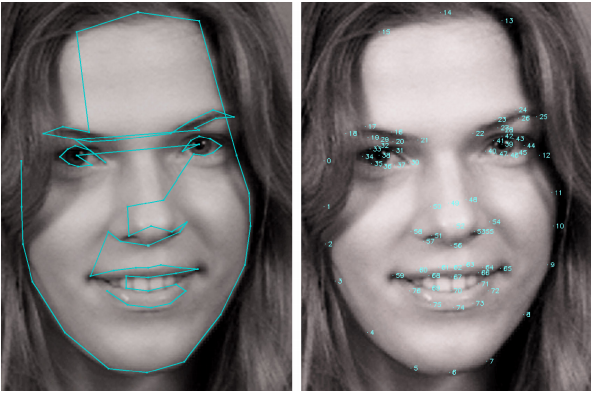
\includegraphics[width=0.7\linewidth]{imagenes/landmarks}
\caption[Puntos de Referencia ASM]{Puntos de Referencia extraídos con ASM.}
\label{fig:landmarks}
\end{figure}


\subsubsection{Facial expression recognition and synthesis based on an appearance model\cite{abboud_davoine_dang04}}
En este caso se hace uso de la técnica \textit{Active Appearance Model (AAM)}\cite{cootes_edwards_taylor98}, un método estadístico que se emplea para emparejar, un modelo geométrico, a una nueva forma del mismo tipo para el que fue entrenado, pero que el modelo no ha visto antes, como por ejemplo un nuevo rostro humano. Esta técnica (AAM)  es una generalización de la ya antes mencionada ASM\cite{cootes_taylor_cooper_graham94}.
Además, lo que en este caso se intenta es que la información usada esté exenta de redundancia por lo que se aplican técnicas de aprendizaje no supervisado en una fase de preprocesamiento de la información como \textit{Análisis de Componentes Principales (PCA)} o \textit{Análisis de Componentes Independientes(ICA)} para reducir la dimensionalidad de la información  en una fase de preprocesamiento. En este caso obtienen alrededor de un 84\% de acierto.

% Una vez descrito el marco general, se explica lo que se quiere hacer con el proyecto con la propuesta concreta que se pretende conseguir.
\subsection{¿Qué se pretende conseguir con este proyecto?}
\label{subsec:aspirations}
\begin{figure}[!]
	\centering
	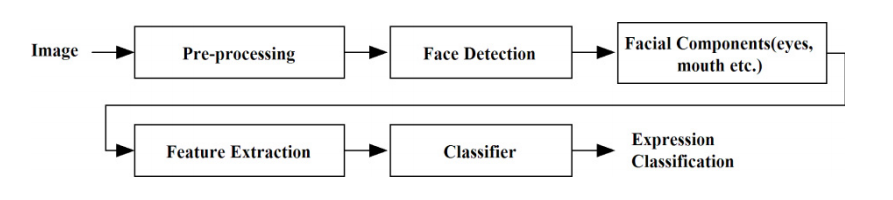
\includegraphics[width=0.7\linewidth]{imagenes/feg_diagram}
	\caption[Diagrama FER]{Diagrama general del proceso de reconocimiento.}
	\label{fig:feg_diagram}
\end{figure}
Las técnicas de ASM\cite{cootes_taylor_cooper_graham94} y AAM\cite{cootes_edwards_taylor98} son sensibles a rotaciones de la imagen, es decir, será difícil extraer los puntos de referencia en imágenes que disten mucho del concepto de imagen frontal, como por ejemplo una la fotografía de una persona mirando hacia un lado con una expresión facial determinada. Además, en la Figura \ref{fig:feg_diagram} extraída del siguiente paper\cite{kumari_rajesh_pooja15}, se puede ver el proceso general que se sigue a la hora de clasificar una imagen, en nuestro caso reconocimiento de expresiones faciales.\\

\begin{figure}[h!]
	\centering
	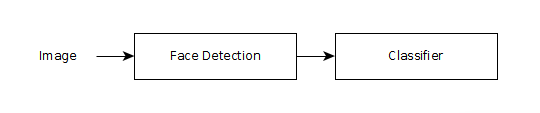
\includegraphics[width=0.7\linewidth]{imagenes/my_fer_diagram}
	\caption[my_diagram]{Diagrama del proceso objetivo.}
	\label{fig:my_fer_diagram}
\end{figure}

La idea principal que se quiere conseguir para resolver el problema consiste en simplificar de alguna manera dicho diagrama para que se asemeje al de la Figura \ref{fig:my_fer_diagram} de forma que no sea necesario extraer características cada vez que se clasifique una nueva imagen. Otra de las propuestas es que la rotación de la imagen de entrada no suponga un hándicap a la hora de clasificarla. El propósito de estas medidas es:\\
\begin{itemize}
	\item Ganar en robustez con imágenes rotadas o inclinadas.
	\item Realizar la clasificación en tiempo real simplificando el preprocesamiento de las imágenes.
	\item Combinar todo en una aplicación de escritorio con una interfaz simple por encima para que cualquier usuario pueda utilizarla.
\end{itemize}

% Se termina explicando la organización de la memoria diciendo lo que se trata en cada capítulo.
\subsection{Organización del documento}
Este documento tratará de explicar el proceso seguido para el desarrollo de este trabajo. Para ello, se estructurará en los siguientes capítulos:\\
\begin{description}
	\item [Portada] - Información básica sobre el nombre del proyecto, la institución, el autor y los tutores.
	\item [Prefacio] - Resumen, palabras clave y agradecimientos.
	\item [Introducción] - Motivación del trabajo y estado del arte de este campo de investigación.  
	\item [Objetivos] - Se planteará un objetivo principal el cual será dividido en sub-objetivos más simples para poder llevar a cabo la tarea principal así como un resumen de las técnicas aprendidas durante la formación académica empleadas en este trabajo.
	\item [Resolución del trabajo] - Este capítulo se dividirá en varias secciones, en las que se explicará el método de ingeniería del software empleado para la resolución del trabajo, así como los recursos hardware y software, la especificación de requisitos, planificación, análisis funcional e implementación de la aplicación.
	\item [Conclusión] - Se hará una valoración del producto final y se valorará si se han alcanzaron o no los objetivos iniciales y en qué medida, teniendo en cuenta los puntos fuertes y débiles de la solución.
	\item [Bibliografía] - Referencias y citas bibliográficas usadas.
	\item [Anexo] - Pequeño manual de cómo usar la aplicación.
\end{description} 

\chapter{Objetivos}
\section{Objetivo principal}
%Objetivo general a conseguir: se enuncia lo que se quiere hacer sin entrar en detalles.
\begin{center}
	\textit{Desarrollar una aplicación de escritorio que dada una imagen detecte si aparece un rostro humano y en que en caso afirmativo, sea capaz de mostrar por pantalla, la etiqueta que mejor identifica la expresión facial que presenta dicho rostro.}\\
\end{center}
Las etiquetas de las expresiones que deseamos predecir son:
\begin{multicols}{2}
	\label{list:expressions}
	\begin{itemize}
		\item Afraid
		\item Angry
		\item Disgusted
		\item Happy
		\item Neutral
		\item Sad
		\item Surprised
	\end{itemize}
\end{multicols}
Se ha de cumplir este objetivo sin olvidar qué es lo que se pretende alcanzar con este trabajo (apartado \ref{subsec:aspirations}). Esto es, simplificar el proceso de pre-procesamiento de las imágenes y de esta forma ver si es factible un proceso de clasificación en tiempo real. Teniendo esto en mente, dividiremos el objetivo principal en distintas fases o sub-tareas.

\section{Objetivos específicos}
% Objetivos específicos: Es dividir el objetivo general en los pasos a seguir con sub-objetivos más simples.
% Dicho de otro modo, son cada uno de los pasos a realizar para alcanzar el objetivo general, es decir solucionando todos y cada uno de los objetivos específicos se resuelve el objetivo general. (Poner entre 3 y 5 como mucho).
%%%%%%%%%%%%%%%%%%%% Se puede decir en qué apartado se tratará cada objetivo específico. %%%%%%%%%%%%%%%%%%%%%%
\begin{enumerate}
	\item Preparación de la información con la que entrenaremos el clasificador.
	\begin{enumerate}
		\item Obtener una base de datos.
		\item Pre-procesamiento de la información.
		\item Creación del conjunto de training, validación y test.
	\end{enumerate}
	\item Entrenamiento del clasificador.
	\begin{enumerate}
		\item Selección de parámetros.
		\item Realización de pruebas (Vuelta al paso 2 si es necesario).
	\end{enumerate}
	\item Desarrollo de interfaz que haga uso del clasificador.
\end{enumerate}

%Poner también los aspectos formativos previos utilizados, por ejemplo si se han usado técnicas de visión concretas como Transformada de Hough, Método de detección de rostros Viola-Jones, Filtro de Partículas, o técnicas de aprendizaje por SVM, etc. Se explica un poco cada método.
\section{Técnicas empleadas}
\label{sec:tecnicas}
Hasta ahora hemos hablado de objetivos, sin entrar demasiado en detalle acerca de qué técnicas serán las que emplearemos para llevarlos a cabo. En la siguiente sección hablaremos sobre ellas, dando una pequeña explicación de su fundamentación teórica.
\subsection{Detector Facial}\label{sub:detectorFacial}
\begin{figure}[t]
	\centering
	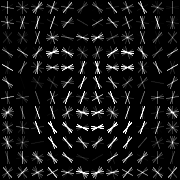
\includegraphics[width=0.3\linewidth]{imagenes/hog01}
	\caption[Descriptores HOG]{Visualización de descriptores HOG en un rostro humano \cite{king14}}
	\label{fig:hog01}
\end{figure}
Dada una imagen, lo primero que necesitamos saber es si aparece un rostro humano o no y en función de ello hacer que nuestra aplicación, actúe de una manera u otra. De esto es de lo que se encarga precisamente un detector facial.\\
Para llevar a cabo esta tarea, el detector facial que he usado ha sido entrenado para aprender mediante un algoritmo basado en \textit{SVM}\cite{cortes_vapnik95} los descriptores de características de una batería de imágenes de rostros humanos previamente marcados y localizados manualmente (Si pudiésemos automatizar el proceso de marcado no necesitaríamos un detector facial). Los descriptores de características aprendidos por el detector son los conocidos como \textit{Histogram of Oriented Gradients (HOG)}\cite{dalal_triggs05} de los que hablaremos a continuación.
\subsubsection{¿Qué es un descriptor de características?}
Es una representación de un conjunto de píxeles, ya sea de una imagen completa o de un trozo de esta. Su misión es simplificar la información que representa una imagen de forma que el descriptor represente la información más útil de la imagen eliminando aquella que no es representativa. 
\subsubsection{Histogram of Oriented Gradients (HOG)}
Hay muchos descriptores de características distintos, pero los que usa nuestro detector son conocidos como descriptores HOG. Estos cuentan las ocurrencias de orientaciones de gradiente en zonas localizadas de una imagen. El gradiente nos indica por cada píxel la magnitud del mayor cambio de intensidad posible y su dirección de oscuro a claro. Podemos observar un ejemplo de esto en la Figura \ref{fig:hog01}.\\
Usando un algoritmo\cite{king15} basado en la técnica de aprendizaje automático conocida como \textit{Support Vector Machine}\cite{cortes_vapnik95}, el detector es capaz de aprender la composición de los descriptores de características HOG de un gran número de caras distintas.\\
Así, dada una imagen, se calculará su descriptor de características y si se encuentra en ella una ventana que contenga descriptores que se asemejen a los aprendidos, habremos detectado satisfactoriamente una cara.

\subsection{Redes Neuronales Convolucionales}\label{sub:cnns}
Tal y como mencioné en la motivación de este trabajo, sin entrar demasiado en detalles, que una de las restricciones de este proyecto era minimizar la fase de pre-procesamiento (apartado \ref{subsec:aspirations}) antes de clasificar una imagen.\\ \\
\begin{figure}[h]
\centering
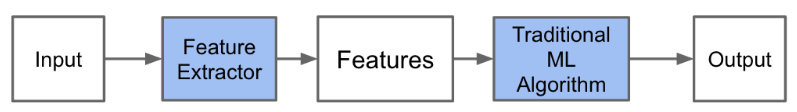
\includegraphics[width=0.7\linewidth]{imagenes/machine_learning_flow}
\caption[Machine Learning]{Esquema general de detección haciendo uso de algoritmos basados en Machine Learning \cite{moujahid16} }
\label{fig:machine_learning_flow}
\end{figure}
\\

Como podemos ver en la Figura \ref{fig:machine_learning_flow} haciendo uso de algoritmos de \textit{Machine Learning} debemos extraer, de la imagen de entrada, una serie de características que la identifiquen, dárselas al algoritmo escogido (previamente entrenado usando un conjunto con esas características) el cual, nos proporcionará una salida en función de lo que el clasificador haya aprendido. Esto supone que los algoritmos clásicos basados en \textit{Machine Learning} son fuertemente dependientes de la representación de las características que se escoja para entrenarlos\cite{bengio_courville_vincent14}. \\ \\
\begin{figure}[h]
	\centering
	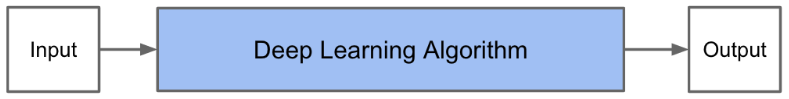
\includegraphics[width=0.7\linewidth]{imagenes/deep_learning_flow}
	\caption[Deep learning]{Detección usando algoritmos basados en Deep Learning \cite{moujahid16}}
	\label{fig:deep_learning_flow}
\end{figure}
\\ \\
Los algoritmos de \textit{Deep Learning} sin embargo nos permiten omitir esa fase de extracción de características, porque han sido diseñados para extraer y abstraer su propia representación de la información a través de la composición de varias transformaciones no lineales\cite{bengio_courville_vincent14}. En nuestro caso, como el problema trata de clasificar imágenes y viendo los buenos resultados obtenidos en los últimos años en problemas de visión por computador\cite{deshpande16}, el algoritmo de \textit{Deep Learning} escogido será el conocido como Redes Neuronales Convolucionales o CNNs. De esta manera, el flujo que se seguiría para realizar la clasificación de una imagen usando CNNs será similar al de la Figura \ref{fig:deep_learning_flow}. Podemos abstraer las CNNs como una caja negra que recibe una imagen de entrada, sin ningún tipo de preprocesamiento previo, y proporciona una etiqueta de salida.\\
\subsubsection{Composición}
\label{subsub:composicion}
Dicho esto, podemos dar una pequeña visión de qué hay dentro de esa caja negra. La arquitectura de una CNN se define como un conjunto de capas conectadas entre si. Hay varios tipos de capas\cite{cs231n} y cada una de ellas realiza una operación específica sobre los datos de entrada que recibe y proporciona unos datos de salida, los cuales que vuelven a ser los datos de entrada para la siguiente capa tal y como podemos observar en la Figura \ref{fig:LeNet}.
\begin{figure}[h]
\centering
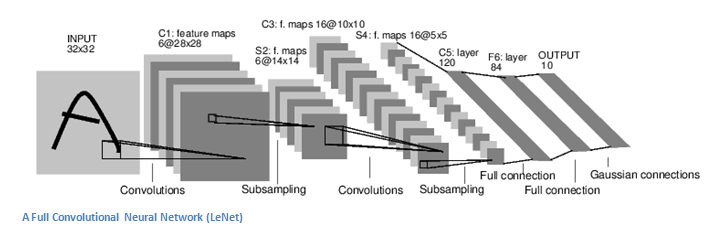
\includegraphics[width=1.0\linewidth]{imagenes/LeNet}
\caption[LeNet]{Arquitectura de Red: LeNet\cite{deshpande16}}
\label{fig:LeNet}
\end{figure}
\subsubsection{Funcionamiento}\label{sub:funcionamientoCnn}
Ahora que conocemos de qué se compone una CNN vamos a ver a grandes rasgos cómo funciona una red neuronal convolucional. Cada una de las capas de las mencionadas en la sección anterior (\ref{subsub:composicion}) se compone a su vez de una serie de neuronas, las cuales tienen unos parámetros, que irán se irán ajustando (aprendiendo) en la fase de entrenamiento de la red, conocidos como pesos. Las neuronas de una capa, estarán solo conectadas con una pequeña región de la capa anterior. De esta forma, a medida que la red va aprendiendo, capas más avanzadas abstraen la información en mayor medida y aprenden patrones más complejos.\\
Dada una imagen de entrada, las neuronas de la red se van activando en función de los patrones aprendidos, y en la última capa calcula la puntuación de que la imagen pertenezca a cada una de las clases para las que la red fue entrenada, dando de esta forma, una etiqueta de salida. Hay muchos tipos de capas que pueden formar la arquitectura de red de una CNN. A continuación veremos un resumen de las más importantes y por norma general, las más usadas.
\begin{description}
	\item [Capas de entrada \cite{cs231n}] - Tal y como su nombre indica, recogen los datos n-dimensionales para la red. Suele ser la primera capa de nuestra arquitectura de red. En nuestro caso, los datos de entrada son las imágenes, que serían elementos tridimensionales teniendo de esta manera un vector del tipo \([ancho \times alto \times profundidad]\). La profundidad puede ser 1 o 3 dependiendo de si la imagen es en color (3 canales RGB) o en escala de grises (1 canal).
	\item [Capas de convolución \cite{cs231n}] - Calcula la salida de neuronas que están conectadas a zonas locales de la imagen de entrada. El valor de cada neurona de salida es el producto escalar entre los pesos de las neuronas de la capa anterior y esa pequeña área local de la imagen. Podemos ver una representación gráfica en la Figura \ref{fig:convolutionlayer}
		\begin{figure}[h]
		\centering
		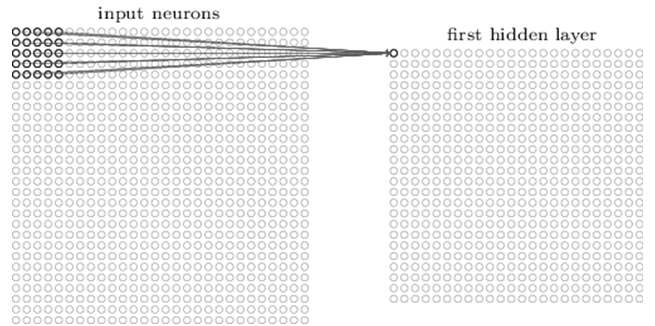
\includegraphics[width=0.7\linewidth]{imagenes/convolutionlayer}
		\caption[Convolution\cite{cs231n}]{Filtro \(5 \times 5\) convolucionando sobre un volumen de entrada\cite{deshpande16}.}
		\label{fig:convolutionlayer}
		\end{figure}
	\item [Capas no lineales o Capas de activación\cite{nair_hinton10,deshpande16b}] - Por convenio, tras una capa de convolución se suele aplicar una capa de activación con el objetivo de añadir \textit{no-linealidad} a un sistema que ha estado haciendo operaciones lineales durante las capas de convolución. Un ejemplo de función no lineal, y una de las más usadas en capas no lineales es:
	\[f(x) = max(0,x)\] 
	También conocida como \textit{Rectified Linear Units} o función \textit{ReLu} que transforma únicamente los valores negativos en cero.
	\item [Capas de submuestreo] - Reduce el tamaño de la imagen a la mitad por norma general. Se pueden aplicar diferentes técnicas para realizar esta operación. Una de las más conocidas se denomina \textit{maxpooling} y podemos ver como funciona en la Figura \ref{fig:poolinglayer}. Esta transformación actúa en las dimensiones espaciales de la imagen (Anchura y Altura).
		\begin{figure}[h]
		\centering
		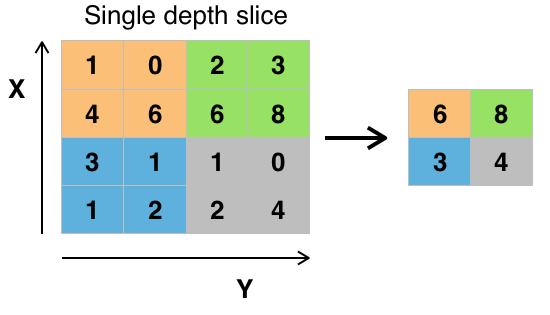
\includegraphics[width=0.7\linewidth]{imagenes/poolinglayer}
		\caption[PoolingLayer]{Reajuste de una imagen \(4\times4\) a una imagen \(2\times2\) usando \textit{maxpooling}\cite{deshpande16b}.}
		\label{fig:poolinglayer}
		\end{figure}
	\item [Capa totalmente conectada\cite{cs231n}] - Esta capa calculará la puntuación de cada clase obteniendo una estructura de salida del tamaño \([1 \times 1 \times n]\) donde \(n\) es el número de clases de salida. En nuestro caso \(n = 7 \) (\ref{list:expressions}).
\end{description}

Este ha sido un pequeño resumen acerca de lo que las redes neuronales convolucionales ofrecen. Es un tema muy extenso el cual no se puede cubrir de forma completa en este documento, además de no ser el objetivo de este. Si se desea saber más acerca de este tema recomiendo el siguiente libro \cite{nielsen}.
\subsubsection{Transfer Learning \cite{cs231n1}}
Se trata de una técnica que se aplica en la fase de entrenamiento de una red neuronal. Consiste en tomar los pesos de un entrenamiento previo como pesos iniciales para nuestro entrenamiento. Dicho de otra manera, es una forma de reutilizar lo que una red neuronal ha podido aprender en otro entrenamiento.\\
Esta técnica es muy útil cuando queremos ahorrar tiempo durante la fase de entrenamiento ya que aumenta la velocidad a la que converge el entrenamiento, o bien cuando el número de imágenes que tenemos es reducido y deseamos reutilizar el trabajo que se ha podido hacer con otras bases de datos.
\subsection{Data Augmentation}
Para nosotros los seres humanos, puede ser muy fácil distinguir una persona sonriendo, aunque esta lleve gafas, tenga o no barba, etc. Pero para una Red Neuronal Convolucional esto no es un hecho automático. Debemos enseñar al modelo, durante la fase de entrenamiento, todas estas posibles variaciones de una misma expresión facial. Debemos mostrarle gente con o sin barba, con o sin gafas, con diferentes condiciones lumínicas, etc. Es por ese motivo que el entrenamiento de una Red Neuronal Convolucional requiere de una gran número de imágenes. \\
Como veremos en el Apartado \ref{db:kdef}, la base de datos que emplearemos para entrenar la red no contiene suficientes imágenes para representar todas estas variaciones de lo que podría ser una imagen de entrada para nuestra aplicación. Hay muchos factores que pueden variar incluso entre dos imágenes del mismo individuo con la misma expresión facial, como por ejemplo:
\begin{itemize}
	\item Diferentes condiciones de luz.
	\item La rotación del rostro con respecto al eje vertical y horizontal de la imagen.
	\item Si el sujeto lleva algún tipo accesorio, como gafas o tiene vello facial.
\end{itemize}
Mientras que hay casos en los que no podemos hacer nada para solucionarlo que no sea obtener otras imágenes distintas, podemos simular algunas de estas variaciones aplicando transformaciones afines y combinaciones de estas a las imágenes de la base de datos, para obtener varias versiones de una misma imagen, que aunque realmente son linealmente dependientes, nos servirán para proporcionar mas variabilidad al modelo. Esta técnica que permite el aumento artificial del conjunto de datos es lo que se conoce como \textit{Data Augmentation}.


\chapter{Resolución del trabajo}
%Como método de ingeniería del software decir que vamos a seguir la técnicas de modelo de prototipos rápido o también llamado modelado de prototipado rápido.
%Ver \url{http://www.ecured.cu/index.php/Modelo_de_Prototipos}catering trade
Dado que el sistema que queremos construir está sujeto a experimentar, como método de ingeniería del software he empleado la técnica de modelo de prototipos rápido o también conocida como modelado de prototipado rápido\cite{ecured_a}.

\section{Recursos}
En esta sección enumeraremos los recursos que han sido utilizados para el desarrollo de este trabajo. Esto incluye recursos humanos como el autor y tutores, hardware y software utilizados así como las bases de datos.
% Decir los recursos humanos (autor y directores), hardware y software que se van a utilizar.
\subsection{Recursos Humanos}
\begin{itemize}
	\item \textbf{Autor}: \myName.
	\item \textbf{Tutor A}: \myProf.
	\item \textbf{Tutor B}: \myOtherProf.
\end{itemize}
\subsection{Recursos Hardware}
Para el desarrollo de este trabajo he empleado mi ordenador personal cuyas especificaciones principales son:
\begin{description}
	\item [CPU] - AMD Phenom(tm) II X4 975
	\item [GPU] - NVidia GTX 760
	\item [Memoria] - 8GB RAM DDR3
\end{description}
\subsection{Recursos Software}\label{sub:software}
Para el desarrollo de la aplicación final, ha hecho falta usar distintas librerías que implementan de una forma eficiente las técnicas descritas en la sección anterior(\ref{sec:tecnicas}), así como distintos frameworks para desarrollar la interfaz de usuario por ejemplo. En la Figura \ref{fig:programming_languages} podemos observar los lenguajes de programación que han sido necesarios para la implementación de esta aplicación.
\\
\begin{figure}[h]
	\centering
	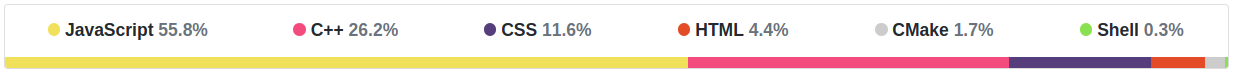
\includegraphics[width=1.0\linewidth]{imagenes/programming_languages}
	\caption[Lenguajes de programación]{Lenguajes de programación que componen la aplicación\cite{franft}.}
	\label{fig:programming_languages}
\end{figure}

\subsubsection{OpenCV \cite{opencv}}\label{sub:opencv}
Por la facilidad de uso que me suponía debido a experiencia previa y su rapidez porque está implementada en C++ e usado esta librería para la manipulación general de imágenes.
\subsubsection{Dlib \cite{dlib}}\label{sub:dlib}
Es una librería que implementa un gran número de algoritmos de Machine Learning en C++. En este caso ha sido usada sólo para el procesamiento de imágenes, pero solo he usado el detector de caras que implementa, el cual he introducido en la Sección \ref{sec:tecnicas}, ya que presentaba menos falsos positivos que el detector de caras de OpenCV\cite{king14}.
\subsubsection{Caffe \cite{caffe}}\label{sub:caffe}
Es un framework de \textit{Deep Learning} implementado en C++ aunque tiene una interfaz en Python. He escogido esta herramienta porque te permite construir tu propia red neuronal, definir tus propias capas de la arquitectura de red, posee buena documentación y buena comunidad. También puedes entrenar y testear tus modelos usando CPU o GPU, además de que ofrece herramientas que facilitan la creación de las bases de datos, todo esto desde la linea de comandos.
\subsubsection{NVIDIA Deep Learning GPU Training System \cite{digits}}\label{sub:digits}
O también conocido como \textit{NVIDIA DIGITS} es un sistema que funciona sobre \textit{Caffe} y que ofrece una interfaz de usuario muy cómoda. Permite ahorrar mucho tiempo en la gestión de diferentes bases de datos, en la recolección de estadísticas de rendimiento de los modelos entrenados. Además simplifica en gran medida la capacidad de entrenamiento con GPU, que mediante linea de comandos puede ser algo difícil de configurar.
\subsubsection{Electron \cite{electron}}\label{sub:electron}
Este framework de código abierto permite crear aplicaciones de escritorio de forma nativa usando tecnologías web como son HTML, JavaScript y CSS. Esto nos permite compatibilidad con diferentes sistemas operativos y desarrollar una interfaz de usuario bonita de forma sencilla.

\subsubsection{Base de datos: Yalefaces \cite{yalefaces}}
Esta base de datos la usé para aprender a manejar herramientas como Caffe y hacer pruebas de clasificación. Aunque no la he usado en la aplicación final, veo necesario hacer una mención a ella.\\
Se compone de 165 imágenes en escala de grises donde se fotografiaron 15 individuos. De cada uno de los individuos hay 11 imágenes, 1 por cada una de las siguientes expresiones básicas:
\textit{Happy, normal, sad, sleepy, surprised, y wink}, además de tener imágenes con luz lateral, central y con gafas tal y como se aprecia en la figura \ref{fig:yalefaceSample}
\begin{figure}[h]
\centering
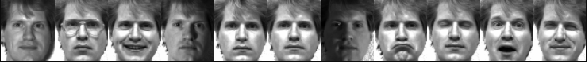
\includegraphics[width=1.0\linewidth]{imagenes/yalefaceSample}
\caption[yafaces]{Muestra de imágenes de la base de datos Yalefaces.}
\label{fig:yalefaceSample}
\end{figure}


\subsubsection{Base de datos: Karolinska Directed Emotional Faces (KDEF) \cite{kdef98}}\label{db:kdef}
\begin{figure}[h]
	\centering
	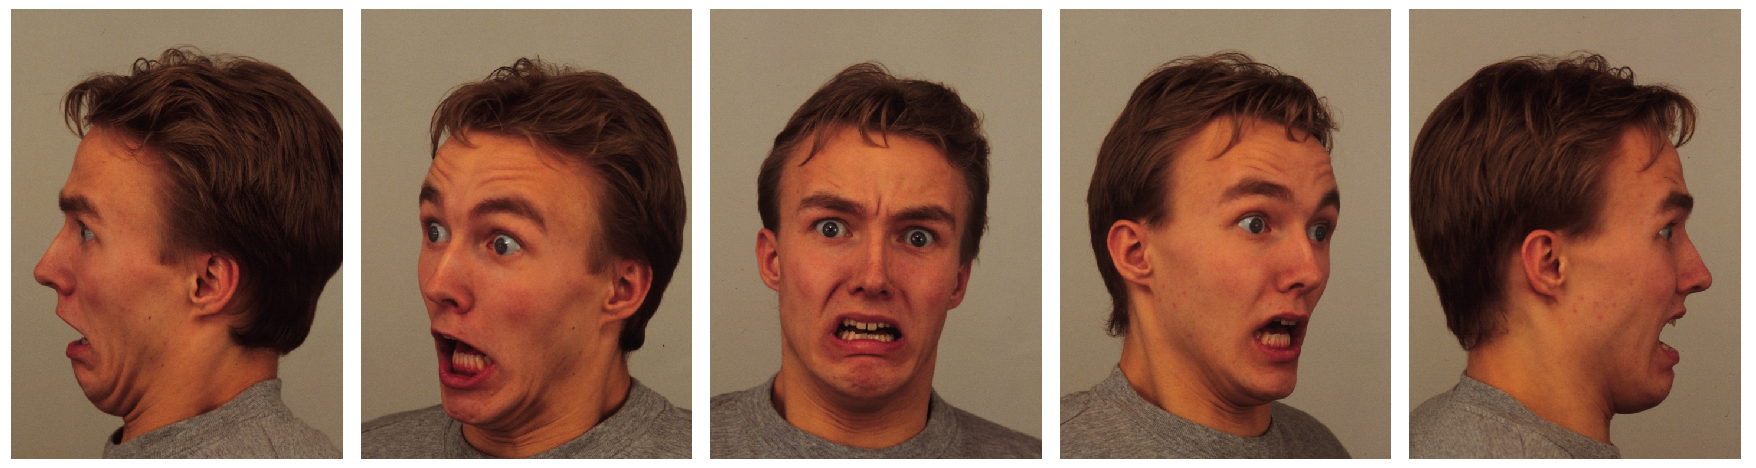
\includegraphics[width=1.0\linewidth]{imagenes/kdefSample}
	\caption[Muestra de KDEF]{Muestra de las imágenes que contiene la base de datos KDEF.}
	\label{fig:kdefSample}
\end{figure}
En este caso estamos ante una base de datos mucho más completa y preparada para el problema que queremos resolver. Esta, recoge imágenes de 70 individuos distintos tomadas desde 5 ángulos diferentes mostrando las 7 expresiones faciales que intentaremos predecir (Sección \ref{list:expressions}).\\
Se realizaron dos sesiones de fotos distintas a todos los individuos, lo que hace un total de 4900 fotografías, en las que se usó una cuadrícula para que la posición de los ojos y la boca de todos los individuos estuviesen siempre en la misma posición. Una muestra de esta base de datos puede verse en la Figura \ref{fig:kdefSample}.

\subsubsection{Resumen}
En la Figura \ref{fig:integracion} se puede ver una visión esquemática de la integración de todas estas tecnologías y en qué fase se usan cada una de ellas.
\begin{figure}[h]
\centering
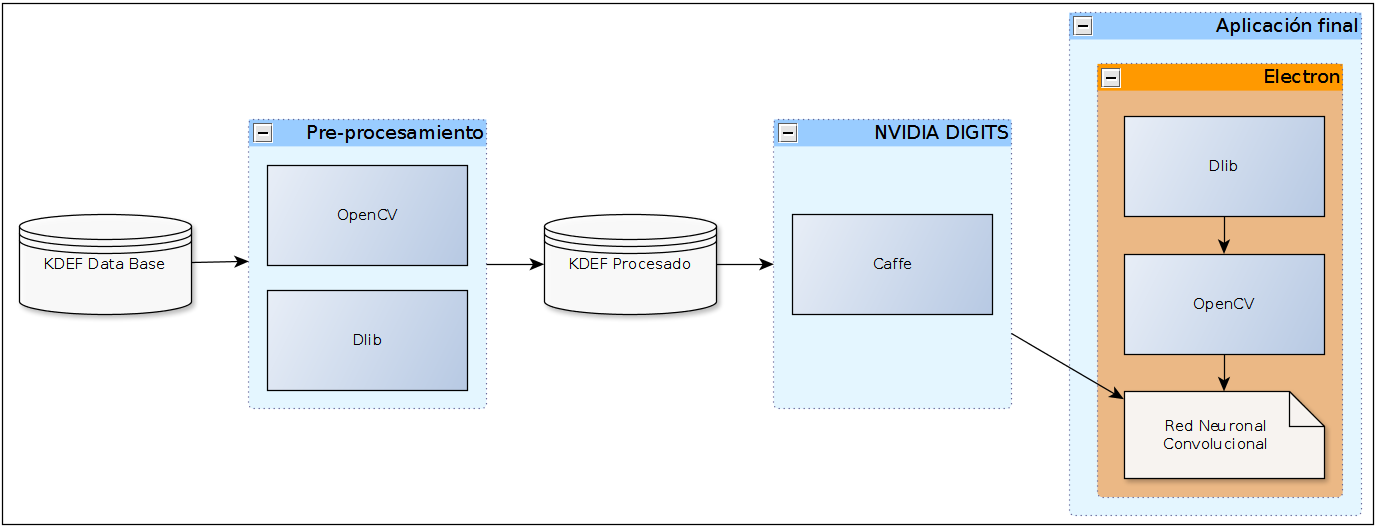
\includegraphics[width=1.0\linewidth]{imagenes/integracion}
\caption[Integración]{Esquema de integración de las distintas tecnologías usadas.}
\label{fig:integracion}
\end{figure}


\section{Especificación de requisitos}

%Decir que se partió de una especificación inicial de requisitos que a medida que se fueron implementando los prototipos se fue refinando posteriormente. Se puede poner la inicial y la final o solo la final indicando que se están poniendo los requisitos que finalmente tiene que tener el sistema.
%Los requisitos se pueden referir a las necesidades del usuario del sistema (requisitos del usuario), a lo que tiene que hacer la aplicación (requisito funcional) o a cómo tiene que hacerlo (requisito no funcional). Ejemplo:

%En este sistema un robot tiene que coger con sus pinzas un envase de medicamento y llevárselo a una persona anciana que por sí misma no puede recordar su medicación.

%Requisitos del usuario:

%rU1. La persona puede moverse libremente por una habitación donde está el robot.

%rU2. La persona es capaz de coger el medicamento cuando se lo ofrece el robot.

%rU3. La persona es capaz de tomarse el medicamento por sí misma.


%Requisitos funcionales.

%rf1. El robot mediante la cámara kinect debe poder localizar a la persona.

%rF2. El robot conoce la posición de la mesa pues tiene un mapa de la habitación.

%rF3. El robot debe identificar el medicamento correcto según un plan de medicación previamente establecido.

%rF4. El robot debe poder coger el medicamento con sus pinzas.

%etc...

%Requisitos no funcionales

%rNF1. El robot no puede atropellar ni dañar a la persona en ningún momento.

%rNF2. La aplicación debe ejecutarse en entornos linux

%rNF3. La aplicación debe utilizar pocos recursos para reaccionar con rapidez.

%algo de la interfaz, como tratar posibles fallos, etc.

En este proyecto se partió de una especificación inicial de requisitos que se fue refinando a medida que se fueron implementando los distintos prototipos. Los requisitos \textbf{finales} son:
\subsection{Requisitos del usuario}
\begin{itemize}
	\item [RU1] El usuario puede seleccionar cualquier fichero de su computador como entrada para la aplicación.
	\item [RU2] El usuario puede arrastrar cualquier fichero a la ventana de la aplicación para proporcionarle una entrada.
\end{itemize}
\subsection{Requisitos funcionales}
\begin{itemize}
	\item [RF1:] La aplicación podrá recibir ficheros de entrada mediante el gestor de ficheros predeterminado del sistema operativo o bien arrastrando el fichero a la ventana principal.
	\item [RF2:] La aplicación solo tendrá en cuenta aquellos ficheros de entrada cuya extensión sean de formatos de imagen válidos: \textit{.png, .jpeg, .jpg}.
	\item [RF3:] La aplicación solo analizará imágenes en las que se encuentren al menos un rostro humano.
	\item [RF4:] El único preprocesamiento que la aplicación realizará sobre la imagen de entrada, será recortar y reajustar el tamaño de la sección en la que se encuentra el rostro.
	\item [RF5:] Una vez clasificada, la aplicación mostrará por pantalla la cara detectada junto a los resultados de su clasificación.
	\item [RF6:] La interfaz notificará al usuario posibles errores mediante una ventana emergente.

\end{itemize}
\subsection{Requisitos no funcionales}
\begin{itemize}
	\item [RNF1:] Para garantizar la validez del fichero de entrada, la aplicación aceptará solo \textit{paths} de imágenes cuya extensión coincida con los formatos de imagen válidos: \textit{png, jpeg, jpg}.
	\item [RNF2:] La aplicación usará el detector de caras de \textit{Dlib} en la imagen de entrada para determinar si hay un rostro humano.
	\item [RNF3:] La ventana emergente de errores indicará:
	\begin{enumerate}
		\item [RNF3.1:] Cuando el fichero de entrada no tiene un formato de imagen válido.
		\item [RNF3.2:] Cuando no se pudo detectar al menos un rostro en la imagen.
		\item [RNF3.3:] Cuando no se seleccionó ningún fichero de entrada.
	\end{enumerate}
	\item [RNF4:] En caso de que la imagen sea válida, es decir en caso de localizar un rostro humano, la aplicación lo recortará y lo reajustará a un tamaño de \([256 \times 256]\) haciendo uso de \textit{OpenCV}. Ese recorte se denominará \textit{imagen intermedia}.
	\item [RNF5:] Para clasificar la \textit{imagen intermedia} se usará un modelo basado en Redes Neuronales Convolucionales previamente entrenado.
	\item [RNF6:] Para mostrar los datos de la clasificación de la \textit{imagen intermedia}, se dibujará un histograma que muestra el porcentaje que tiene la imagen intermedia de contener una expresión determinada. El histograma tendrá un máximo de 5 resultados y será dibujado usando HTML y JavaScript.
	\item [RFN7:] El histograma no mostrará por pantalla los resultados en los que el porcentaje de acierto es inferior al 1\%.
	\item [RFN8:] El histograma mostrará una animación donde los porcentajes van creciendo hasta alcanzar su valor.	
\end{itemize}

\section{Planificación}

%Poner una tabla de tiempos con las planificación del proyecto diciendo cuando se tiene previsto alcanzar cada subobjetivo planteado. Con su correspondiente división en fases y tareas, y la posterior comparación con los datos reales obtenidos tras realizar el proyecto. Entre las fases está la realización de los diferentes prototipos I, II y III por ejemplo.

%Poner presupuesto según horas de trabajo estimadas.

En la tabla \ref{tab:planificacion} están dispuestos, de forma aproximada, los tiempos estimados y empleados en cada uno de los principales sub-objetivos. \\
Como se puede observar, el prototipo I es el que más tiempo ha consumido. Esto es porque era el punto de inicio, lo que implica tener que empezar de cero, aprender conceptos teóricos sobre temas que solo conocía de oídas como por ejemplo las Redes Neuronales Convolucionales (Apartado \ref{sub:cnns}) a usar nuevas tecnologías que las implementaban como Caffe (Apartado\ref{sub:caffe}) además del resto como puede ser OpenCV (Apartado\ref{sub:opencv}) mediante la realización de ejemplos para entenderlas de forma correcta. El prototipo I además no constaba con interfaz, se manejaba todo por línea de comandos y algunos scripts en shell bash.\\

\newcolumntype{P}[1]{>{\centering\arraybackslash}p{#1}} % Nuevo tipo de columna: Párrafo centrado.
\begin{table}[h]
	\centering
	\label{tab:planificacion}
	\begin{tabular}{lc|P{2cm}|P{2cm}|P{2cm}|}
		\cline{3-5}
		\multicolumn{2}{l}{}                                  				& \multicolumn{3}{|c|}{\textbf{T. empleado} por prototipo} \\ \hline
		\multicolumn{1}{|p{3cm}|}{\textbf{Sub-objetivo}} 					&  \textbf{T. estimado} 	& \textbf{I}	& \textbf{II} & \textbf{III} \\ \hline
		\multicolumn{1}{|p{3cm}|}{\textbf{Preparación de la información}}	& \(\sim 1\) mes & \(\sim 2\) meses & \(\sim 7\) días & \(\sim 5\) días \\ \hline
		\multicolumn{1}{|p{3cm}|}{\textbf{Entrenamiento del clasificador}}	& \(\sim 2\) meses & \(\sim 3\) meses & \(\sim 1\) mes & \(\sim 7\) días \\ \hline
		\multicolumn{1}{|p{3cm}|}{\textbf{Desarrollo de la interfaz}}		& \(\sim 2\) meses & - & \(\sim 1\) mes & - \\ \hline
	\end{tabular}
	\caption{Planificación de tiempos sub-objetivos. Nota:\textit I, II y III equivale al número de prototipo. }
\end{table}

En el prototipo II, ya tenía asentados los conocimientos aprendidos mediante la implementación del primer prototipo, lo que agilizó el desarrollo del segundo prototipo. Este se basó en mejorar los resultados del entrenamiento de la Red Neuronal Convolucional mediante nuevas técnicas de pre-procesado sobre las imágenes y haciendo test con distintos parámetros de entrenamiento, pero se reutilizaban muchas de las herramientas implementadas en el prototipo I. El descubrimiento de NVIDIA DIGITS (Apartado \ref{sub:digits}) también ayudó en gran medida a la reducción de este tiempo gracias al aprovechamiento de la GPU para la fase de entrenamiento. En este prototipo además implementé la interfaz, que llevó menos tiempo del esperado debido a la sencillez que aporta Electron (Apartado \ref{sub:electron}) para el desarrollo de interfaces.\\
En el último prototipo es una versión mejorada del segundo en el que se mejora la precisión del clasificador dejando la interfaz intacta.

\section{Análisis funcional}
% A partir de aquí nos referimos solamente al prototipo final que da lugar a la aplicación final.

% Hay que describir la funcionalidad que debe poseer el sistema para poder cumplir con los objetivos y requisitos que se han dicho previamente.La descripción de esta funcionalidad puede hacerse analizando las tareas (que aparecerán en la planificación) y estudiando la inter-relación entre ellas y sus conexiones.

%Para la realización de este análisis se pueden utilizar Diagramas de Flujo para poder conocer generalmente un único punto de inicio y un único punto de término o en varios.

%\url{https://es.wikipedia.org/wiki/Diagrama_de_flujo}

La aplicación tiene que ser capaz de obtener un fichero de entrada, comprobar si es válido y en caso afirmativo proceder a la clasificación de este usando el modelo previamente entrenado.\\
En la Figura \ref{fig:appFlowchart} se ilustra el comportamiento de la aplicación final en función de los posibles casos que se pueden dar durante la ejecución. Los rectángulos verdes indican la ejecución de sub-procesos. El que se encuentra más arriba de los dos en la Figura \ref{fig:appFlowchart}, es el único que realiza algún tipo de preprocesamiento en la imagen que se quiere clasificar, y lo único que hace es generar el recorte de la cara. Este era uno de los principales objetivos como se comentó en el Apartado \ref{subsec:aspirations}.
\begin{figure}[t]
\centering
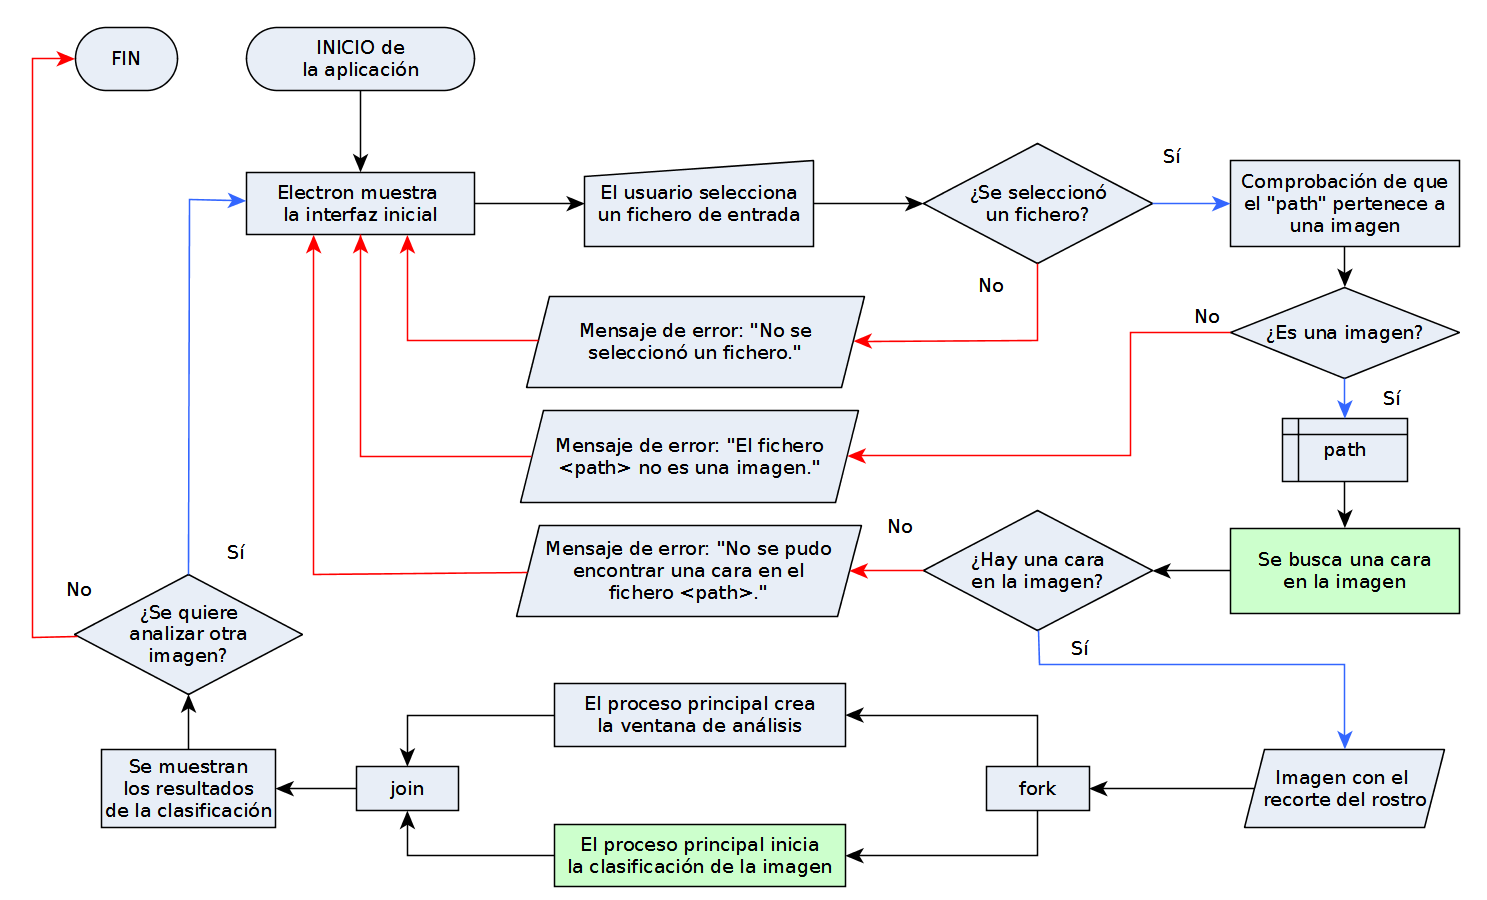
\includegraphics[width=1.0\linewidth]{imagenes/appFlowchart}
\caption[FlowChart]{Diagrama de flujo de la aplicación final.}
\label{fig:appFlowchart}
\end{figure}



%Se pueden plantear también casos de uso. Los diagramas de casos de uso sirven para describir la inter-relación entre el sistema y el usuario del mismo. Se pueden utilizar para plantear diferentes casos de interacción entre el robot y la persona y cómo tiene que reaccionar el sistema en cada caso.

%\url{https://es.wikipedia.org/wiki/Diagrama_de_casos_de_uso}
\begin{figure}[t]
	\centering
	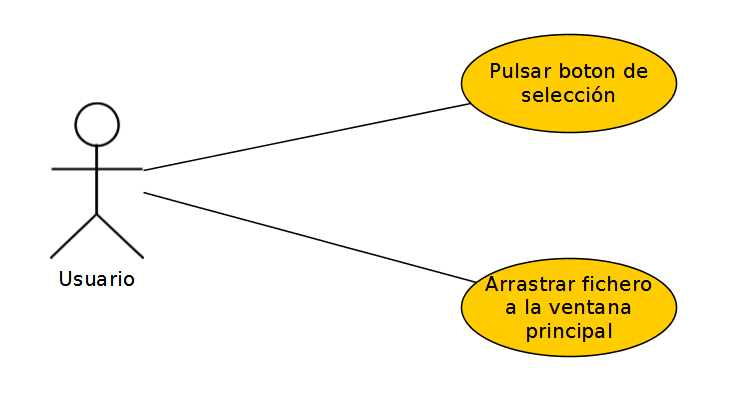
\includegraphics[width=0.7\linewidth]{imagenes/usecases}
	\caption[Casos de uso.]{Casos de uso}
	\label{fig:usecases}
\end{figure}

Aunque la inter-relación entre el usuario y la aplicación es muy simple, pueden darse varios casos de uso de la aplicación a la hora de proporcionar el fichero de entrada. Como se puede ver en la Figura \ref{fig:usecases} el usuario puede proporcionar el fichero mediante el uso del botón de selección presente en la interfaz, que abre el gestor de archivos por defecto del S.O. Si se da este caso, no haría falta comprobar que el fichero es una imagen porque el propio gestor te permite filtrar por tipos de archivo y solo he permitido la selección de archivos con un formato de imagen válido.\\
El otro caso es que el usuario arrastre directamente el fichero a la ventana. En esta ocasión si sería necesario comprobar que el fichero tiene una extensión de archivo válida ya que ha podido arrastrar cualquier tipo de fichero.\\
Como se puede ver la aplicación final no es demasiado compleja. La complejidad de este trabajo reside en entrenar una Red Neuronal Convolucional para obtener la máxima precisión posible, tema que abordaremos de lleno en la siguiente sección.



\section{Implementación y pruebas}

%Decir qué lenguaje de programación se ha utilizado y las tecnologías implicadas aunque se hayan comentado en el apartado de recursos. Justificar su uso (rendimiento, disponibilidad, etc.). Si se ha usado open source decirlo y explicar las ventajas.
Los lenguajes de programación que más he utilizado han sido \textit{C++, HTML, CSS, JavaScript y Bash} como se puede aprecia en la Figura \ref{fig:programming_languages}. Aunque este último ha sido empleado en gran parte durante la implementación de los primeros prototipos para su gestión de ficheros en el S.O. En el Apartado \ref{sub:software} se presentó cada una de ellas pero en esta sección hablaremos un poco más a fondo sobre su uso en la implementación de la aplicación.\\
Si vemos la aplicación como un conjunto de capas, empezaremos a describir cómo están integradas estas tecnologías de arriba hacia abajo, siendo este el orden:
\begin{enumerate}
	\item Interfaz
	\item Módulo de clasificación.
	\item Entrenamiento del clasificador.
\end{enumerate}

\subsection{Interfaz}\label{sub:interfaz}
\textit{HTML, CSS y JavaScript} siempre han estado asociados al ámbito de las tecnologías web. Con estos lenguajes, se consiguen desarrollar interfaces de usuario de forma muy cómoda y rápida en el lado del cliente de forma que:
\begin{itemize}
	\item HTML se usa para la estructura.
	\item CSS se usa para el aspecto.
	\item JavaScript se usa para la funcionalidad.
\end{itemize}
Por mi experiencia en este campo, sabía que si lograba integrar estos tres lenguajes con mi funcionalidad principal, implementada en C++, conseguiría tener una aplicación de escritorio que pudiese funcionar en diversos sistemas operativos de una forma rápida con un aspecto más que notable. Además tendremos la estructura de nuestra interfaz, su estilo y su funcionalidad de forma separada, por lo que, si queremos cambiar el aspecto de la misma, por ejemplo, simplemente habrá que cambiar la hoja de estilos CSS.\\
Es entonces cuando encontré \textbf{Electron} (Apartado \ref{sub:electron}), un framework \textbf{open source} que hacía posible integrar estos lenguajes asociados a las tecnologías web, HTML, CSS y JavaScript en una aplicación de escritorio, justo lo que buscaba.\\
Internamente Electron, crea un proceso principal que es el que tiene permisos para hacer llamadas al S.O. ya sea para lectura de ficheros, creación de directorios, etc. A su vez, crea sub-procesos que renderizarán las distintas ventanas de nuestra aplicación. El proceso principal y sus sub-procesos se comunican de forma asíncrona mediante el envío y la recepción de mensajes.\\
De esta forma el proceso principal puede proporcionar información que requiera uno de sus sub-procesos y que este no pueda conseguir porque no tiene acceso a llamadas al S.O. o bien obtener resultados al ejecutar sub-módulos, como por ejemplo, los resultados de clasificar una imagen.\\
La interfaz en sí es concisa y no pretende ser complicada. Permite al usuario seleccionar un fichero mediante un botón de \textit{selección de fichero}. Este es capturado por el proceso que renderiza la ventana de la interfaz, y le envía al proceso principal un mensaje asíncrono para que realice una llamada al S.O que invoca al gestor de archivos por defecto y le aplica unos filtros para permitir solamente que el usuario pueda seleccionar imágenes.\\
Una vez el proceso principal obtiene el path del archivo, este se pasa al módulo de clasificación para que realice las pertinentes operaciones con las imágenes, lo cual veremos en el siguiente apartado. Cuando el proceso principal obtiene los datos de salida del módulo de clasificación, este se los pasa al sub-proceso para renderizarlos en pantalla.\\
Hasta este punto nuestra aplicación estaría de la siguiente manera tal cual se ve en la Figura \ref{fig:interfaz}, una interfaz que recoge un path.
\begin{figure}[h]
\centering
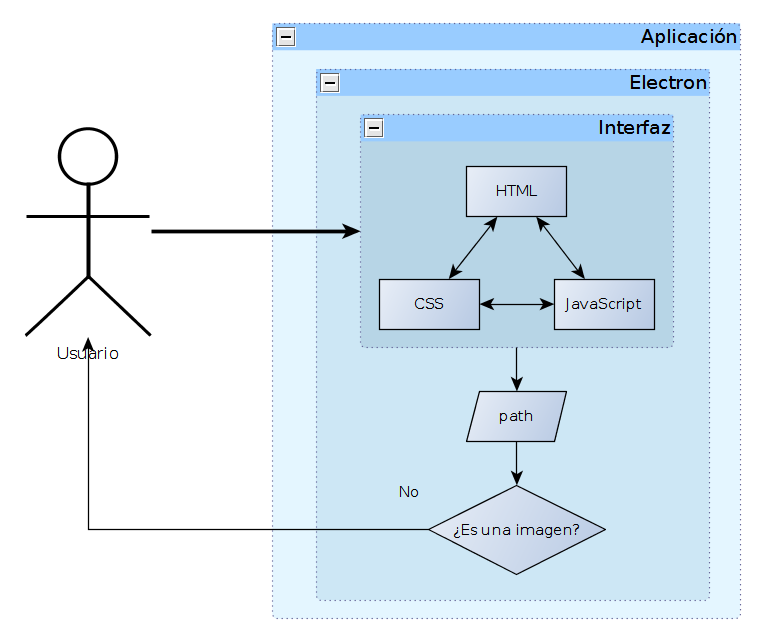
\includegraphics[width=0.9\linewidth]{imagenes/interfaz}
\caption[Interfaz]{Composición parcial de la aplicación (1/3).}
\label{fig:interfaz}
\end{figure}


\subsection{Módulo de clasificación}
Desde un principio quería que la aplicación funcionara en torno a C++ ya que es uno de los lenguajes con mayor rendimiento, característica que es de interés si se está pensando en un sistema que trabaje en tiempo real en un futuro, además de ser el lenguaje que más he usado durante mi paso por la \myUni y con el que me sentía más cómodo.\\
Teniendo esto en cuenta, busqué herramientas que estuviesen implementadas en este lenguaje que me pudiesen ayudar a resolver el problema del entrenamiento de una red neuronal convolucional, clasificar una imagen, detectar rostros en imágenes, etc. Este fue uno de los motivos por el que me decanté a usar herramientas como \textbf{OpenCV} (Apartado \ref{sub:opencv}) o \textbf{Caffe} (Apartado \ref{sub:caffe}) entre otras, ambas implementadas en C++, pero no el único.\\
La parte de la aplicación que se dedica al análisis y la gestión de la imagen de entrada es el Módulo de clasificación, y tal y como he mencionado antes, es conveniente que sea lo más rápida posible, asique está implementada en C++. El módulo de clasificación consta de dos sub-módulos:

\begin{enumerate}
	\item El primero de ellos recibe el path de la imagen seleccionada por el usuario mediante la interfaz (Apartado \ref{sub:interfaz}) y comprueba que aparezca al menos una cara. En caso afirmativo, realiza un recorte de esa cara y lo guarda como una imagen de tamaño \([256\times256]\). Si no se encuentra una cara no se clasifica la imagen.\\
	Esta herramienta está implementada en C++ y usa OpenCV y Dlib  (Apartado \ref{sub:opencv}). Ambas librerías son open source. Podría haberse usado solamente OpenCV ya que también incluye un detector pero el que implementa Dlib (Apartado \ref{sub:detectorFacial}) genera menos falsos positivos \cite{king14}.
	\item El segundo sub-módulo es el que se encarga de clasificar el recorte del rostro obtenido antes. Para ello hemos tenido que entrenar y generar previamente un modelo basado en Redes Neuronales Convolucionales que sea capaz de dicha tarea. Aquí es donde entra en juego Caffe (Apartado \ref{sub:caffe}).\\
	Como ya mencioné es un framework de deep learning, open source implementado en C++ que nos permite definir nuestra propia arquitectura de red, nuestras propias capas, realizar entrenamientos tanto en CPU como en GPU y ofrece un gran conjunto de herramientas, como por ejemplo, dado un modelo entrenado, generar una clasificación ante una información de entrada. Esto es justo este segundo sub-módulo.
\end{enumerate}

El estado de la aplicación en este momento es el que se muestra en la Figura \ref{fig:moduloClasificacion} pero nos sigue faltando lo más importante, el clasificador que veremos cómo ha sido obtenido en la siguiente sección.
\begin{figure}[h]
\centering
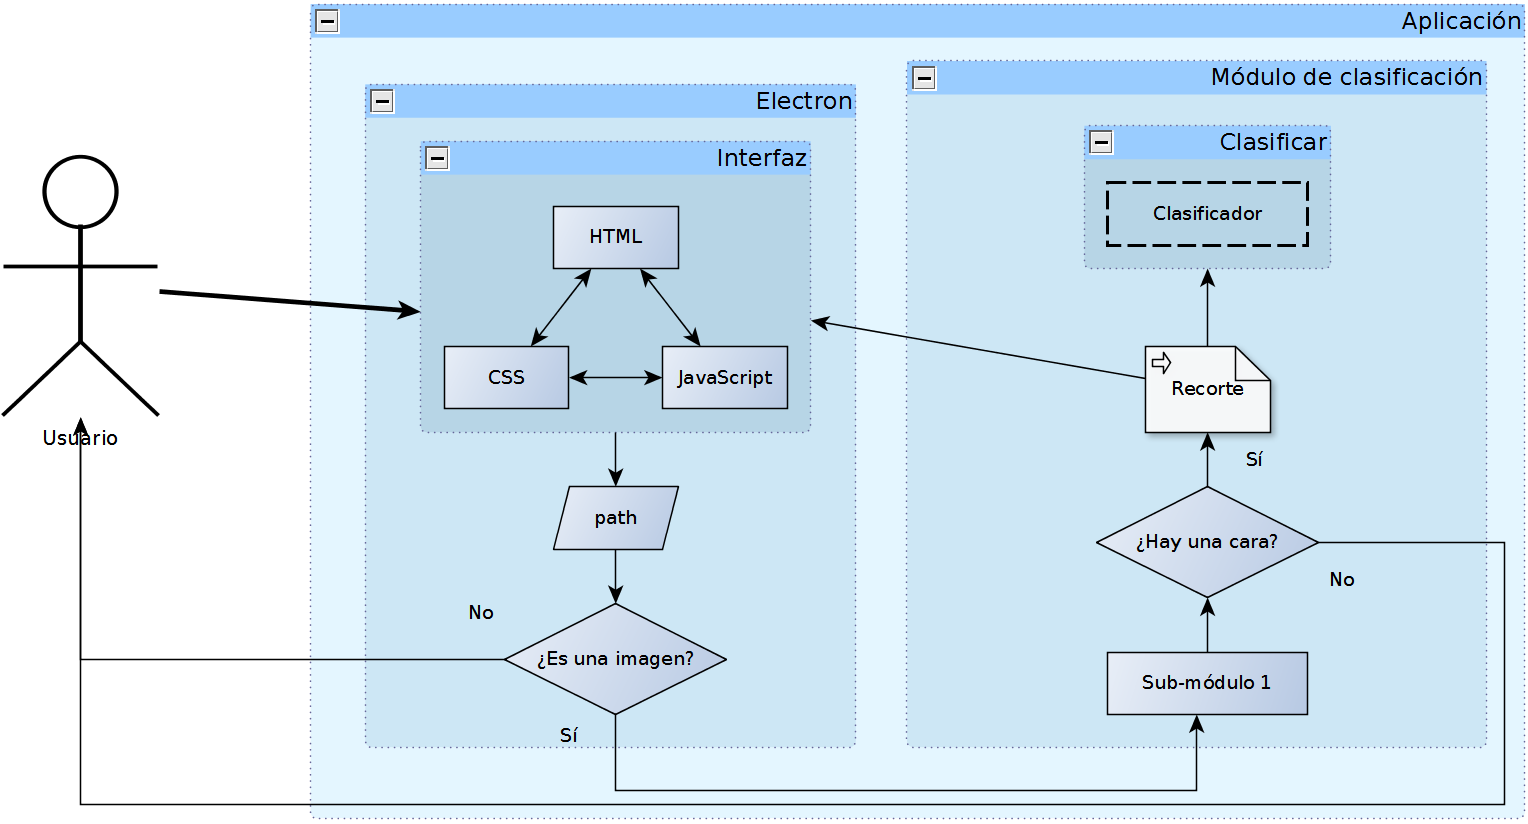
\includegraphics[width=0.9\linewidth]{imagenes/moduloClasificacion}
\caption[Módulo de Clasificación]{Aplicación con interfaz y módulo de clasificación (2/3).}
\label{fig:moduloClasificacion}
\end{figure}


\subsection{Entrenamiento del clasificador}
Para que el módulo de clasificación funcione correctamente debemos entrenar un clasificador basado en redes neuronales convolucionales. En esta ocasión podríamos usar Caffe por si solo, pero decidí usar NVIDIA DIGITS (Apartado \ref{sub:digits}) porque simplifica el proceso permitiéndonos centrarnos en lo que realmente importa, la fase de entrenamiento. NVIDIA DIGITS funciona sobre Caffe, aunque también soporta otros frameworks, y ofrece una interfaz sencilla e intuitiva que permite gestionar todos los modelos, todos los conjuntos de datos y recoge de forma automática métricas útiles durante el entrenamiento.

\subsubsection{Arquitectura de Red}

\begin{figure}[h]
\centering
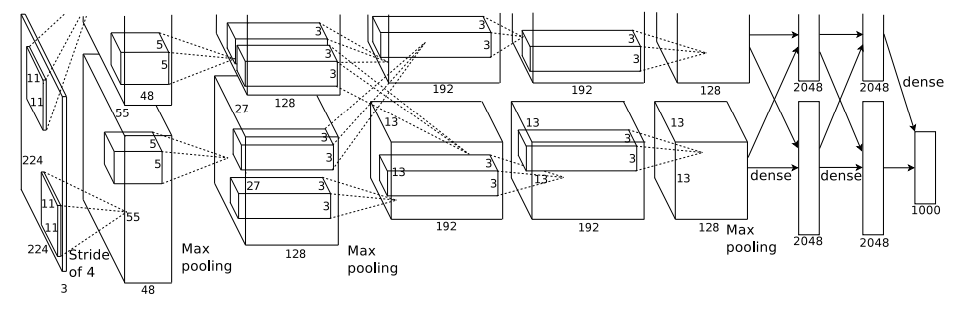
\includegraphics[width=1\linewidth]{imagenes/alexNet}
\caption[AlexNet]{AlexNet\cite{krizhevsky12}}
\label{fig:alexNet}
\end{figure}
El primer paso para entrenar un modelo es comenzar escogiendo o formando una arquitectura de red. En mi caso, he escogido AlexNet\cite{krizhevsky12}(Figura \ref{fig:alexNet}), conocida por su buen rendimiento en el concurso de ImageNet LSVRC-2010 que consistía en clasificar \(1,2M\) de imágenes entre \(1000\) clases diferentes.
Contiene 8 capas de aprendizaje, distribuidas como 5 capas de convolución y 3 capas totalmente conectadas (Apartado \ref{sub:funcionamientoCnn}).\\

\begin{figure}[h]
\centering
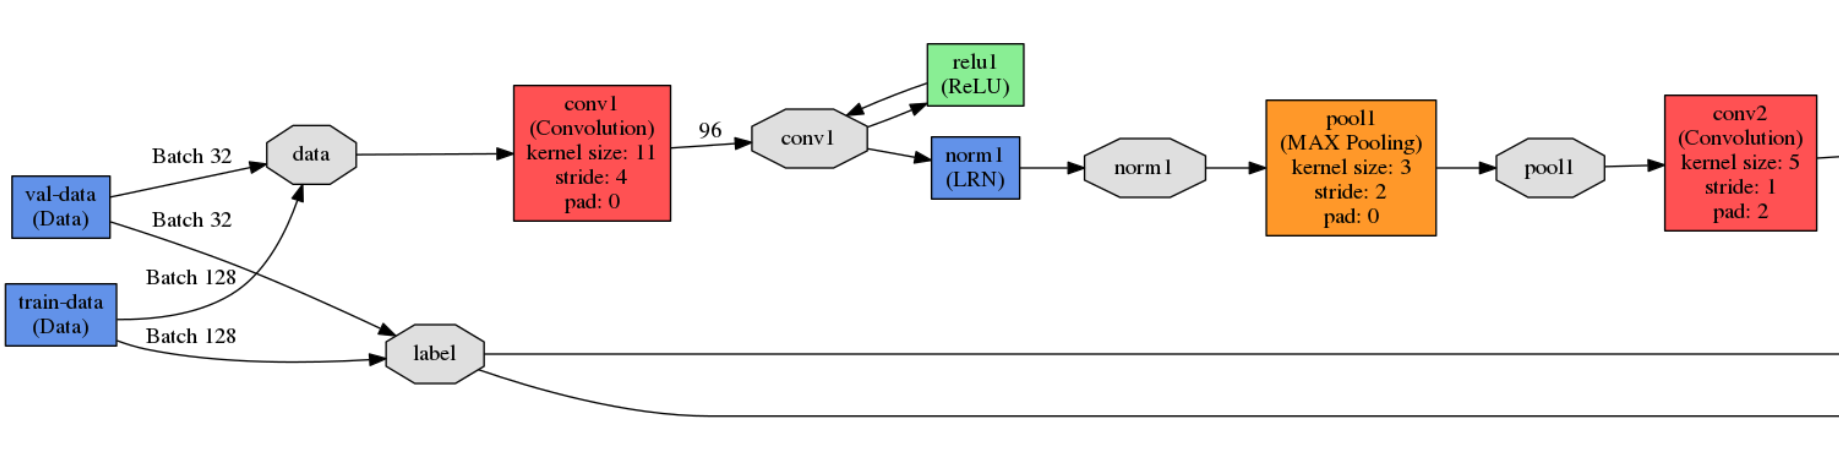
\includegraphics[width=1\linewidth]{imagenes/alexNet1}
\caption[AlexNet input]{Primeras capas de AlexNet}
\label{fig:alexNet1}
\end{figure}

En la Figura \ref{fig:alexNet1} se puede observar el primer conjunto de capas de nuestra arquitectura. Vemos como la primera capa obtiene los datos de entrada, \textit{validation} y \textit{training}, que llegan a la primera capa de convolución. Concretamente en esta capa, se puede observar que se obtienen 96 filtros de salida, calculados sobre las imágenes de entrada con un tamaño del kernel de convolución de \(11\times11\) y un stride de 4.\\
A la salida de la capa de convolución se le añade no-linealidad aplicándoles la función Rectified Linear Units o ReLu (ver Apartado \ref{sub:funcionamientoCnn}). En las redes neuronales convencionales se añadía no-linealidad usando la función:
\begin{center}
	\(f(x) = \tanh(x)\) o bien \(f(x) = (1+e^{-x})^{-1}\)
\end{center}
En esta arquitectura se usa la función ReLu con el objetivo de aumentar la velocidad de entrenamiento sin sacrificar demasiado en rendimiento del clasificador. Acto seguido se normalizan los datos mediante Local Response Normalization o LRN de las 2 primeras capas de convolución, ya que se ha probado que el modelo gana en generalización\cite{krizhevsky12}, y se le aplica una capa de submuestreo. Este es el esquema general de la arquitectura de red para las capas de convolución.\\

\begin{figure}[h]
	\centering
	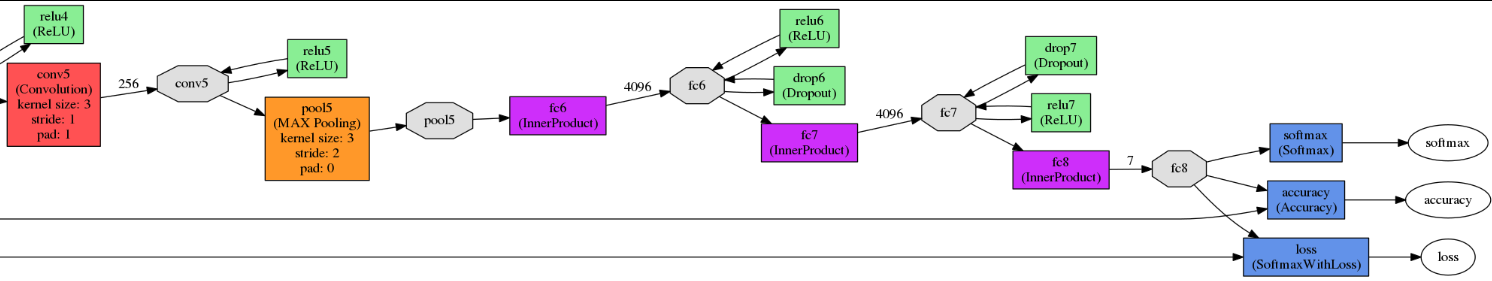
\includegraphics[width=1\linewidth]{imagenes/alexNet2}
	\caption[AlexNet input]{Últimas capas de AlexNet}
	\label{fig:alexNet2}
\end{figure}

Luego se conecta lá última capa de convolución con la primera de las tres capas totalmente conectadas, como se puede ver en la Figura \ref{fig:alexNet2}, para comenzar a calcular los scores de cada clase y finalmente obtener la etiqueta de salida. Para reducir el sobreajuste en las capas totalmente conectadas se aplica una capa de Dropout una técnica que permite mejorar el rendimiento del clasificador que consiste en poner a cero la salida de cada una de las neuronas ocultas con una probabilidad del 50\%, para que no participen en el proceso de \textit{fordward pass} y de \textit{back propagation}\cite{krizhevsky12}.

\subsubsection{Base de datos}
Una vez se tiene una arquitectura de red, debemos conseguir una base de datos con la que poder entrenarla. En mi caso, y como ya mencioné en el Apartado \ref{db:kdef} de Recursos, la base de datos que he podido conseguir es: \textit{Karolinska Directed Emotional Faces (KDEF)} \cite{kdef98}.\\
Para cada entrenamiento debemos dividir esa base de datos en dos conjuntos a los que llamaremos:
\begin{itemize}
	\item \textbf{Conjunto de entrenamiento o de training}: Es el conjunto que se usa para el aprendizaje de la red neuronal. 
	\item \textbf{Conjunto de validación}: Es el conjunto que se usa para verificar si la red neuronal está aprendiendo o no.
\end{itemize}
Por último decir que para medir el rendimiento real del clasificador es necesario otro conjunto de datos externo a la base de datos. A este conjunto lo llamaremos \textbf{conjunto de test}.

\section{Fase de entrenamiento}
En este apartado veremos las distintas pruebas que he realizado, y cómo ha ido evolucionando el clasificador ante distintos parámetros de entrenamiento. Véase que el conjunto de imágenes de test siempre será de un total de 140 imágenes escogidas al azar que no tienen nada que ver con la base de datos empleada para el entrenamiento.
\subsection{Primer Intento}\label{sub:entrenamiento1}
Este primer intento es una toma de contacto para probar la herramienta NVIDIA DIGITS por lo que el conjunto de imágenes es muy pequeño.
\subsubsection{Base de datos}
Para este primer intento he cogido simplemente las caras frontales de la base de datos, dejando a un lado las laterales.

\subsubsection{Preprocesamiento}
Para cada una de las imágenes escogidas de la base de datos:
\begin{itemize}
	\item He recortado el mismo rectángulo a todas las imágenes para obtener un recorte de los rostros centrado, ya que los sujetos que aparecen en la base de datos KDEF tienen los ojos en las mismas coordenadas.
	\item He reajustado la imagen resultante del recorte a un tamaño de \(256\times256\ \).
\end{itemize}
Con esto, he obtenido una batería de imágenes como las de la Figura \ref{fig:primerIntentoDB}.

\begin{figure}[h]
\centering
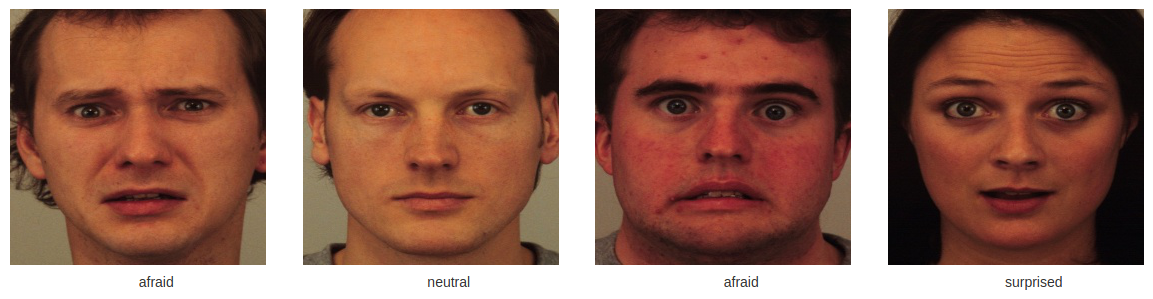
\includegraphics[width=0.7\linewidth]{imagenes/primerIntentoDB}
\caption[PrimerIntentoDB]{Muestra de imágenes empleadas para el primer intento de entrenamiento.}
\label{fig:primerIntentoDB}
\end{figure}

Tras el preprocesamiento, se ha separado el conjunto de imágenes en los dos subconjuntos mencionados anteriormente, training y validación. El tamaño de ambos conjuntos se muestra en la tabla \ref{entr:PrimerIntento-DB}.\\
Véase que los subconjuntos de training y validación \textbf{deben estar balanceados} para que los resultados del entrenamiento tengan validez. En este caso el conjunto de training tiene 105 imágenes por cada clase mientras que el conjunto de validación tiene 35 imágenes.

\begin{table}[h]
	\centering
	\begin{tabular}{c|c|c|c|}
		\cline{2-4}
		& \textbf{Training} & \textbf{Validación} (25\%) & \textbf{Total} \\ \hline
		\multicolumn{1}{|c|}{\textbf{Nº de imágenes}} & 735        & 245          & 980     \\ \hline
	\end{tabular}
	\caption{DB empleada - Primer intento}
	\label{entr:PrimerIntento-DB}
\end{table}

\subsubsection{Parámetros de entrenamiento}
\begin{itemize}
	\item Epochs: \(100\)
	\item Coeficiente de aprendizaje inicial: \(0.02\)
	\item Policy: Sigmoid (Figura \ref{fig:entrenamiento1results1})
\end{itemize}

\subsubsection{Resultados del entrenamiento}
Como podemos ver en los resultados Figura \ref{fig:entrenamiento1results}, con el paso de los epochs o épocas, la precisión del clasificador ha ido mejorando. Esto se puede ver en como la línea naranja tiene una tendencia positiva. También podemos observar como a partir de los 70 epochs aproximadamente, el modelo converge y no mejora.\\

\begin{figure}[h]
\centering
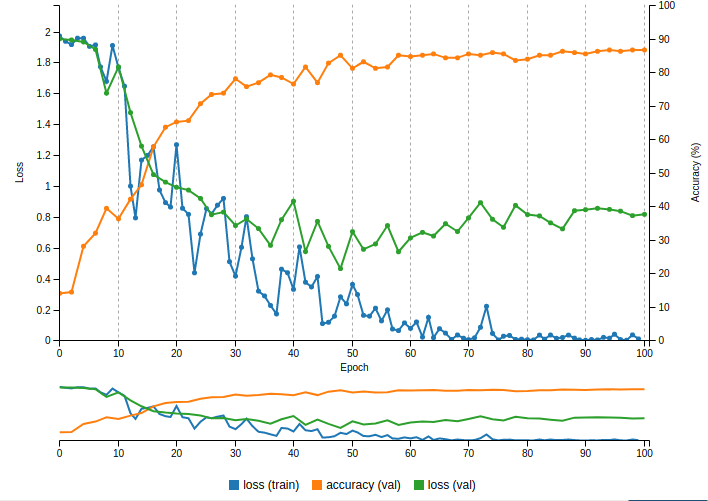
\includegraphics[width=0.9\linewidth]{imagenes/entrenamiento1results}
\caption[Resultados del entrenamiento 1]{Resultados del primer entramiento. Linea naranja: Precisión para el conjunto de validación. Linea verde: Función de pérdida para el conjunto de validación. Linea azul: Función de perdida para el conjunto de training.}
\label{fig:entrenamiento1results}
\end{figure}
La función de pérdida (loss) tanto para training como para validación comienza disminuyendo de forma exponencial en las primeras épocas hasta que se estabiliza y no oscila tanto como al principio. Esto es debido a que el coeficiente de entrenamiento va disminuyendo también (Figura \ref{fig:entrenamiento1results1}), por lo que el modelo tiende a converger. Podemos interpretar esta función de pérdida como \textit{cúanto le queda por aprender a nuestro modelo} ya sea del conjunto de training (linea azul) o validación (linea verde).\\
También podemos observar en la Figura \ref{fig:entrenamiento1results} como a partir de la mitad del entrenamiento, la función de pérdida del conjunto de validación cambia su tendencia descendente para comenzar a aumentar. Esto puede significar que estamos empezando a sobreajustar el modelo porque la función de pérdida para training es prácticamente 0.

\begin{figure}[h]
	\centering
	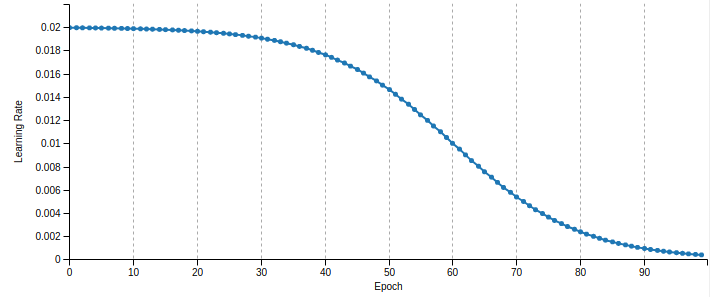
\includegraphics[width=0.9\linewidth]{imagenes/entrenamiento1results1}
	\caption[Resultados del entrenamiento 1]{Política de disminución del coeficiente de aprendizaje.}
	\label{fig:entrenamiento1results1}
\end{figure}

Para medir el rendimiento real del clasificador, debemos clasificar el conjunto de test y cuantificar los aciertos y los errores que se han cometido. Esto se conoce como calcular la matriz de confusión.\\

\begin{table}[h]
	\centering
	\small
	\setlength\tabcolsep{3pt}
	\setlength\extrarowheight{2pt}
	\begin{tabular}{lccccccclc}
		& \multicolumn{1}{l}{\textbf{afraid}} & \multicolumn{1}{l}{\textbf{angry}} & \multicolumn{1}{l}{\textbf{disgusted}} & \multicolumn{1}{l}{\textbf{happy}} & \multicolumn{1}{l}{\textbf{neutral}} & \multicolumn{1}{l}{\textbf{sad}} & \multicolumn{1}{l}{\textbf{surprised}} &  & \multicolumn{1}{l}{\textbf{per-class}} \\
		\textbf{afraid}    & \cellcolor[HTML]{EFEFEF}13 & 1	& 1 & 0 & 0 & 4 & 1 &  & 65,00\% \\
		\textbf{angry}     & 17 & \cellcolor[HTML]{EFEFEF}1 & 0 & 0 & 1 & 1 & 0 &  & 5,00\% \\
		\textbf{disgusted} & 9 & 1 & \cellcolor[HTML]{EFEFEF}0 & 0 & 0 & 10 & 0 &  & 0,00\% \\
		\textbf{happy}     & 9 & 1 & 0 & \cellcolor[HTML]{EFEFEF}3 & 2 & 5 & 0 &  & 15,00\% \\
		\textbf{neutral}   & 10 & 0 & 0 & 0 & \cellcolor[HTML]{EFEFEF}3 & 7 & 0 &  & 15,00\% \\
		\textbf{sad}       & 8 & 0 & 1 & 0 & 1 & \cellcolor[HTML]{EFEFEF}8 & 2 &  & 40,00\% \\
		\textbf{surprised} & 16 & 0 & 0 & 0 & 0 & 0 & \cellcolor[HTML]{EFEFEF}4 &  & 20,00\%
	\end{tabular}
	\caption{Matriz de confusión}
	\label{tab:entrenamiento1MC}
\end{table}

Tras clasificar el conjunto de test, la matriz de confusión de este primer modelo es la que se muestra en la tabla \ref{tab:entrenamiento1MC}. Podemos ver en la matriz como los aciertos ocuparán las casillas en gris, el resto son fallos. Como vemos el clasificado tiene un rendimiento muy pobre y ha obtenido un porcentaje de acierto en el conjunto de test del 22,86\% pese a tener un 87,00\% de acierto con el conjunto de validación. Era de esperar viendo el reducido número de imágenes con el que hemos entrenado el clasificador.

%Las pruebas se realizan para comprobar la verificación y validación del producto software. La verificación consiste es comprobar que el producto realiza lo que está programado, es decir la programación no tiene errores y funciona en todos los casos cumpliendo los requisitos. La validación tiene que ver con que cumpla con lo que espera el usuario.

%Verificación y Validación: Conjunto de procesos de comprobación y
%análisis que aseguran que el software que se desarrolla está acorde a su
%especificación y cumple las necesidades de los clientes.

%Verificación:
%¿Estamos construyendo el producto correctamente?
%Se comprueba que el software cumple los requisitos funcionales y no funcionales
%de su especificación.

%Validación:
%¿Estamos construyendo el producto correcto?
%Comprueba que el software cumple las expectativas que el cliente espera
%Importante: Nunca se va a poder demostrar que el software está
%completamente libre de defectos

%las pruebas que pueden utilizarse son muy diversas. Aconsejo centrarnos en pruebas de caja blanca y de caja negra.

%Las pruebas de la caja blanca se centran en la estructura interna del programa para elegir los casos de prueba. El objetivo de estas pruebas consiste en probar todos los posibles casos de ejecución de la aplicación para comprobar que los datos se comportan de manera correcta internamente.

%Decir que se han hecho las pruebas de caja blanca.

%Las pruebas de caja negra son aquellas que se centran en las salidas y entradas de los módulos, sin atender a su comportamiento interno (comprobando mediante las pruebas de caja blanca). Las pruebas de caja negra garantizan la interconectividad entre los diferentes módulos de la aplicación, así como su correcto funcionamiento final.

%Poner algunos casos de prueba de caja negra.

\chapter{Conclusiones y trabajo futuro}

Decir lo que se ha conseguido realizar comentando sus puntos fuertes y débiles.
Decir si se han alcanzado los objetivos específicos y el general propuesto y en qué grado.

Indicar las asignaturas del grado más relacionadas con la ejecución del TFG y cómo el TFG ha ayudado a afianzar los conocimientos adquiridos en el Grado.

Valoración personal si se quiere.


Avanzar algunas líneas de trabajo futuro para solucionar las debilidades detectadas o para conseguir nuevas funcionalidades interesantes.

\chapter{Bibliografía}
%% Poner las citas bibliográficas, direcciones de internet, etc.
\begin{thebibliography}{99}
	\section{Artículos científicos}
	%%%%%%%%%%%%%%%%%%
	%%%%% Papers %%%%%
	%%%%%%%%%%%%%%%%%%
	\bibitem{shbib_zhou15}
	R. Shbib, and S. Zhou. %Names
	\textit{Facial Expression Analysis using Active Shape Model}, %Title
	School of Engineering, University of Portsmouth, United Kingdom	%Location
	2015.	%Date
	
	\bibitem{abboud_davoine_dang04}
	B. Abboud, F. Davoine, and M. Dang. %Names
	\textit{Facial expression recognition and synthesis based on
		an appearance model}, %Title
	Heudiasyc Laboratory CNRS, University of Technology of Compiegne, BP 20529, 60205 Compiegne Cedex, France	%Location
	2004.	%Date
	
	\bibitem{cootes_taylor_cooper_graham94}
	T. F. Cootes, C. J. Taylor, D. H. Cooper, and J. Graham. %Names
	\textit{Active Shape Models - Their Training and Application}, %Title
	Department of Medical Biophysics, University of Manchester, Oxford Road, Manchester M13 9PT, England 	%Location
	1994.	%Date
	
	\bibitem{cootes_edwards_taylor98}
	T. F. Cootes, G. J. Edwards, and C. J. Taylor. %Names
	\textit{Active Appearance Models}, %Title
	Wolfson Image Analysis Unit, Department of Medical Biophysic, University of Manchester, Manchester M13 9PT, UK %Location
	1998.	%Date
	
	\bibitem{kumari_rajesh_pooja15}
	J. Kumari, R. Rajesh, and KM. Pooja. %Names
	\textit{Facial expression recognition: A survey}, %Title
	Dept. of Computer Science, Central University of South Bihar, India 
	2015.	%Date
	
	\bibitem{dalal_triggs05}
	N. Dalal, and B. Triggs. %Names
	\textit{Histograms of Oriented Gradients for Human Detection}, %Title
	INRIA Rhône-Alps, 655 avenue de l’Europe, Montbonnot 38334, France
	2005.	%Date
	
	\bibitem{king15}
	D. E. King.
	\textit{Max-Margin Object Detection}, %Title
	arXiv:1502.00046 [cs.CV],
	2015.	%Date
	
	\bibitem{cortes_vapnik95}
	C. Cortes, and V. Vapnik. %Names
	\textit{Support Vector Networks}, %Title
	Kluwer Academic Publishers, Boston. Manufactured in The Netherlands,
	1995.	%Date
	
	\bibitem{bengio_courville_vincent14}
	Y. Bengio, A. Courville, and Pascal. Vincent. %Names
	\textit{Representation Learning: A Review and New Perspectives}, %Title
	Department of computer science and operations research, U. Montreal 
	also, Canadian Institute for Advanced Research (CIFAR),
	2014.	%Date
	
	\bibitem{nair_hinton10}
	V. Nair, and G. E. Hilton. %Names
	\textit{Rectified Linear Units Improve Restricted Boltzmann Machines}, %Title
	Department of Computer Science, University of Toronto, Toronto, ON M5S 2G4, Canada
	2010.	%Date
	
	\bibitem{krizhevsky12}
	NIPS2012\_4824,
	Alex Krizhevsky and Sutskever, Ilya and Hinton, Geoffrey E. %Names
	\textit{ImageNet Classification with Deep Convolutional Neural Networks}, %Title
	Advances in Neural Information Processing Systems 25, by %Book
	F. Pereira and C. J. C. Burges and L. Bottou and K. Q. Weinberger, pages 1097-1105,%editor
	Curran Associates, Inc.
	URL: \url{http://papers.nips.cc/paper/4824-imagenet-classification-with-deep-convolutional-neural-networks.pdf}
	2012.	%Date
	
	\section{URLs}
	%%%%%%%%%%%%%%%%
	%%%%% URLS %%%%%
	%%%%%%%%%%%%%%%%
	\bibitem{king14}
	D. King. 
	\textit{Dlib 18.6 released: Make your own object detector!}, 
	URL: \url{http://blog.dlib.net/2014/02/dlib-186-released-make-your-own-object.html}, 
	2014.
	
	\bibitem{moujahid16}
	A. Moujahid. 
	\textit{A Practical Introduction to Deep Learning with Caffe and Python}, 
	URL: \url{http://adilmoujahid.com/posts/2016/06/introduction-deep-learning-python-caffe/}, 
	2016.
	
	\bibitem{deshpande16}
	A. Deshpande. 
	\textit{A Beginner's Guide To Understanding Convolutional Neural Networks}, 
	URL: \url{https://adeshpande3.github.io/adeshpande3.github.io/A-Beginner%27s-Guide-To-Understanding-Convolutional-Neural-Networks/}, 
		2016.
		
	\bibitem{deshpande16b}
	A. Deshpande. 
	\textit{A Beginner's Guide To Understanding Convolutional Neural Networks - Part 2}, 
	URL: \url{https://adeshpande3.github.io/adeshpande3.github.io/A-Beginner's-Guide-To-Understanding-Convolutional-Neural-Networks-Part-2/}, 
	2016.
	
	\bibitem{cs231n}
	CS231n  
	\textit{Convolutional Neural Networks for Visual Recognition}, 
	URL: \url{http://cs231n.github.io/convolutional-networks/}.
	
	\bibitem{nielsen}
	M. Nielsen,   
	\textit{Neural Networks and Deep Learning}, 
	URL: \url{http://neuralnetworksanddeeplearning.com/}.
	
	\bibitem{ecured_a}
	Ecu Red Conocimiento con todos y para todos,   
	\textit{Modelo de Prototipos}, 
	URL: \url{http://www.ecured.cu/index.php/Modelo_de_Prototipos}.
	
	\bibitem{franft}
	F. Fajardo,   
	\textit{Face Expression Detector}, 
	Repositorio GitHub del proyecto, 
	URL: \url{https://github.com/FranFT/Face-Expression-Detector}, 
	2017
	
	\bibitem{cs231n1}
	CS231n  
	\textit{Convolutional Neural Networks for Visual Recognition: Transfer Learning}, 
	URL: \url{http://cs231n.github.io/transfer-learning/}.
	
	
	\section{Herramientas}
	%%%%%%%%%%%%%%%%%
	%%%%% Tools %%%%%
	%%%%%%%%%%%%%%%%%
	\bibitem{opencv}
	\textit{OpenCV}, 
	URL: \url{http://opencv.org/}.
	
	\bibitem{dlib}
	\textit{Dlib}, 
	URL: \url{http://dlib.net/}.
	
	\bibitem{caffe}
	\textit{Caffe}, 
	URL: \url{http://caffe.berkeleyvision.org/}.
	
	\bibitem{digits}
	\textit{NVIDIA DIGITS}, 
	URL: \url{https://developer.nvidia.com/digits}.
	
	\bibitem{electron}
	\textit{Electron}, 
	URL: \url{https://electron.atom.io/}.
	
	\section{Bases de datos}
	%%%%%%%%%%%%%%%%%%%%%
	%%%%% Databases %%%%%
	%%%%%%%%%%%%%%%%%%%%%
	\bibitem{yalefaces}
	\textit{Yalefaces Database}, 
	URL: \url{	http://cvc.cs.yale.edu/cvc/projects/yalefaces/yalefaces.html}.
	
	\bibitem{kdef98}
	Lundqvist, D., Flykt, A., \& Öhman, A. (1998). %Names
	\textit{The Karolinska Directed Emotional Faces - KDEF}, %Title
	CD ROM from Department of Clinical Neuroscience, Psychology section, Karolinska Institutet, ISBN 91-630-7164-9
	
	

	
\end{thebibliography}
\chapter{Anexo}

Al final de la memoria hay que añadir un anexo de una página o dos, explicando como se usa el software a modo de manual de usuario. Es decir, como se llaman los comandos, qué parámetros hay que darle, como se llaman los ficheros de datos de entrada, etc.



%
%\input{capitulos/02_EspecificacionRequisitos}
%
%\input{capitulos/03_Planificacion}
%
%\input{capitulos/04_Analisis}
%
%\input{capitulos/05_Diseno}
%
%\input{capitulos/06_Implementacion}
%
%\input{capitulos/07_Pruebas}
%
%\input{capitulos/08_Conclusiones}
%
%%\chapter{Conclusiones y Trabajos Futuros}
%
%
%%\nocite{*}
%\bibliography{bibliografia/bibliografia}\addcontentsline{toc}{chapter}{Bibliografía}
%\bibliographystyle{miunsrturl}
%
%\appendix
%\input{apendices/manual_usuario/manual_usuario}
%%\input{apendices/paper/paper}
%\input{glosario/entradas_glosario}
% \addcontentsline{toc}{chapter}{Glosario}
% \printglossary
\chapter*{}
\thispagestyle{empty}

\end{document}
